\documentclass[14pt, a4paper]{article}
\usepackage{minitoc}
\usepackage[left=3.00cm, right=2.5cm, top=2.00cm, bottom=2.00cm]{geometry}
\usepackage{amsmath}
\usepackage{amssymb}
\usepackage{amsthm}
\usepackage{mathtools}
\usepackage{graphicx}
%\usepackage{algpseudocode}
%\usepackage{algorithm}
\usepackage[ruled,vlined,linesnumbered]{algorithm2e}
\usepackage{blindtext}
\usepackage{setspace}
\usepackage[utf8]{inputenc}
\usepackage[utf8]{vietnam}
\usepackage[center]{caption}
\usepackage[shortlabels]{enumitem}
\usepackage{fancyhdr} % header, footer
\usepackage{hyperref} % loại bỏ border với mục lục và công thức
\usepackage[nonumberlist, nopostdot, nogroupskip]{glossaries}
\usepackage{glossary-superragged}
\usepackage{tikz,tkz-tab}
\usepackage{pythonhighlight}
\usepackage{float}
\setglossarystyle{superraggedheaderborder}
\pagestyle{fancy}
%\usepackage[style=numeric,sortcites]{biblatex}
%\addbibresource{ref.bib}
%\usepackage[numbers]{natbib}
\usepackage{indentfirst}
\usepackage[natbib,backend=biber,style=ieee, sorting=ynt]{biblatex}

\usepackage{caption}
\usepackage{subcaption}

\bibliography{ref.bib}

\graphicspath{{./figures/}}

\fancyhf{}
%\rhead{\textbf{Môn học: Các phương pháp thống kê hiện đại trong nghiên cứu Xã hội học}}
\lhead{\textbf{GVHD: TS. Trịnh Quốc Anh}}
\rfoot{\thepage}
\lfoot{\textbf{Học viên thực hiện: Nguyễn Chí Thanh - 21007925}}
\renewcommand{\headrulewidth}{0.4pt}
\renewcommand{\footrulewidth}{0.4pt}
%
%\numberwithin{equation}{section}
%\numberwithin{algorithm}{section}
%\numberwithin{figure}{section}
%
%\setlength{\parindent}{0.5cm}
%
%\setcounter{secnumdepth}{3} % Cho phép subsubsection trong report
%\setcounter{tocdepth}{3} % Chèn subsubsection vào bảng mục lục

%\newtheorem{dl}{Định lý}
%\newtheorem{md}{Mệnh đề}
%\newtheorem{bd}{Bổ đề}
%\newtheorem{dn}{Định nghĩa}
%\newtheorem{hq}{Hệ quả}

%\newtheorem{baitap}{Bài tập}
%\newtheorem*{loigiai}{Lời giải}

%\numberwithin{dl}{section}
%\numberwithin{md}{section}
%\numberwithin{bd}{section}
%\numberwithin{dn}{section}
%\numberwithin{hq}{section}

\setlength{\parindent}{0cm}

\newtheorem{dl}{Định lý}
\newtheoremstyle{sltheorem}
{}                % Space above
{}                % Space below
{\normalfont}        % Theorem body font % (default is "\upshape")
{}                % Indent amount
{\bfseries}       % Theorem head font % (default is \mdseries)
{.}               % Punctuation after theorem head % default: no punctuation
{ }               % Space after theorem head
{}                % Theorem head spec
\theoremstyle{sltheorem}
\newtheorem{baitap}{Bài tập}
\newtheoremstyle{soltheorem}
{}                % Space above
{}                % Space below
{\normalfont}        % Theorem body font % (default is "\upshape")
{}                % Indent amount
{\bfseries}       % Theorem head font % (default is \mdseries)
{.}               % Punctuation after theorem head % default: no punctuation
{\newline}               % Space after theorem head
{}                % Theorem head spec
\theoremstyle{soltheorem}
\newtheorem*{loigiai}{Lời giải}

\onehalfspacing


\begin{document}
\begin{titlepage}

    \newcommand{\HRule}{\rule{\linewidth}{0.5mm}} % Defines a new command for the horizontal lines, change thickness here

    \center % Center everything on the page

    %----------------------------------------------------------------------------------------
    %	HEADING SECTIONS
    %----------------------------------------------------------------------------------------
    \textsc{\LARGE Đại học Quốc Gia Hà Nội}\\[0.5cm]
    \textsc{\LARGE Trường đại học Khoa học tự nhiên}\\[0.5cm] % Name of your university/college
    \textsc{\LARGE Khoa Toán - Cơ - Tin học}\\[0.5cm]

    
\includegraphics[scale=0.2]{HUS-logo.jpg}\\[0.5cm]

    \textsc{\Large Chuyên ngành: Khoa học dữ liệu}\\[0.5cm] % Major heading such as course name


    %----------------------------------------------------------------------------------------
    %	TITLE SECTION
    %----------------------------------------------------------------------------------------

    \HRule \\[0.4cm]
    { \huge \bfseries Bài tập môn học}\\[0.4cm] % Title of your document
    \HRule \\[1.5cm]

    \textsc{\Large Môn học: Các phương pháp thống kê hiện đại \\ trong nghiên cứu Xã hội học}\\[1cm] % Minor heading such as course title


    \textsc{\Large Bài tập giữa kỳ}\\[1cm]


    %----------------------------------------------------------------------------------------
    %	AUTHOR SECTION
    %----------------------------------------------------------------------------------------
    \begin{minipage}{0.4\textwidth}
        \begin{flushleft} \large
        \emph{Giảng viên hướng dẫn:} \\
        TS. Trịnh Quốc Anh % Supervisor's Name
        \end{flushleft}
    \end{minipage}\\[0.5cm]

    \begin{minipage}{0.4\textwidth}
    \begin{flushleft} \large
    \emph{Học viên thực hiện:}\\
    Nguyễn Chí Thanh \\
    MSHV: 21007925 \\ % Your name
    Lớp: Khoa học dữ liệu - K4
    \end{flushleft}
    \end{minipage}


    % If you don't want a supervisor, uncomment the two lines below and remove the section above
    %\Large \emph{Author:}\\
    %John \textsc{Smith}\\[3cm] % Your name

    %----------------------------------------------------------------------------------------
    %	DATE SECTION
    %----------------------------------------------------------------------------------------

    % I don't want day because it is English
    % {\large \today}\\[2cm] % Date, change the \today to a set date if you want to be precise

    %----------------------------------------------------------------------------------------
    %	LOGO SECTION
    %----------------------------------------------------------------------------------------

    %\includegraphics{logo/rsz_3logo-khtn.png}\\[1cm] % Include a department/university logo - this will require the graphicx package

    %----------------------------------------------------------------------------------------

    \vfill % Fill the rest of the page with whitespace

\end{titlepage}

\nocite{*}

\newpage

\begin{baitap}
    Ước lượng Bayes cho tham số của phân phối Poisson.

    Đính kèm là dữ liệu tổng điều tra xã hội (GSS) của Mỹ từ năm 1972 đến năm 1998.

    Người ta quan tâm đến số con trung bình (tỷ lệ sinh) của phụ nữ Mỹ ở độ tuổi 40 trong thập niên 1990 (YEAR$\geq$1990 \& AGE==40 \& FEMALE==1). 
    Có 02 nhóm phụ nữ được nghiên cứu là nhóm có trình độ văn hoá trên phổ thông (DEG$\geq$3) và nhóm còn lại. 
    Biết rằng số con sinh ra tuân theo phân phối Poisson.
    
    Từ dữ liệu và sử dụng thống kê Bayes, hãy:

    \begin{enumerate}
        \item Xác định phân phối của dữ liệu (likelihood)
        \item Xác định phân phối hậu nghiệm của tỷ lệ sinh khi phân phối tiên nghiệm là:
        \begin{enumerate}[label=(\alph*)]
            \item Phân phối đều
            \item Phân phối Gamma
        \end{enumerate}
        \item Nêu đặc điểm của các phân phối hậu nghiệm tìm được
        \item Ước lượng tỷ lệ sinh của 02 nhóm phụ nữ
        \item So sánh tỷ lệ sinh của 2 nhóm và đánh giá sự khác biệt (nếu có)
    \end{enumerate}
\end{baitap}

\begin{loigiai}

    \textbf{1. Phân tích tập dữ liệu:}

    Ta xét tập dữ liệu:

    \begin{figure}[H]
        \centering
        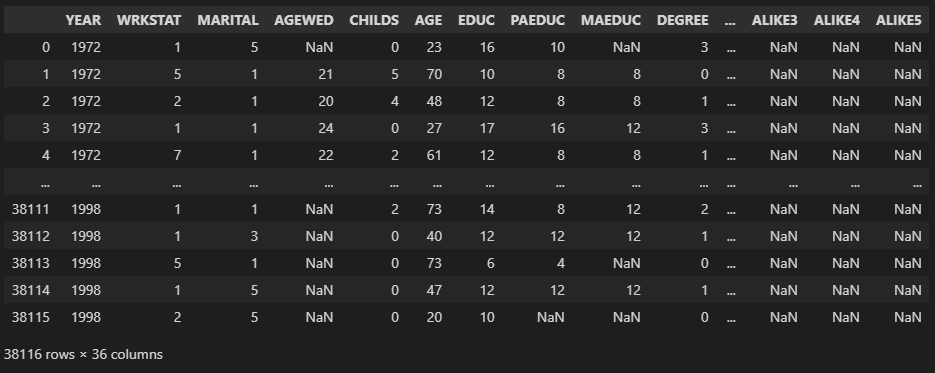
\includegraphics[width=0.8\linewidth]{figures/overall_df.png}
        \caption{Dataframe của tập dữ liệu}
        \label{fig:overall_df}
    \end{figure}

    Tập dữ liệu gồm 38116 hàng và 36 trường dữ liệu.
    Số trường dữ liệu khá lớn, ta sẽ chỉ quan tâm tới một số trường dữ liệu có ý nghĩa khá dễ hiểu.

    \begin{figure}[H]
        \centering
        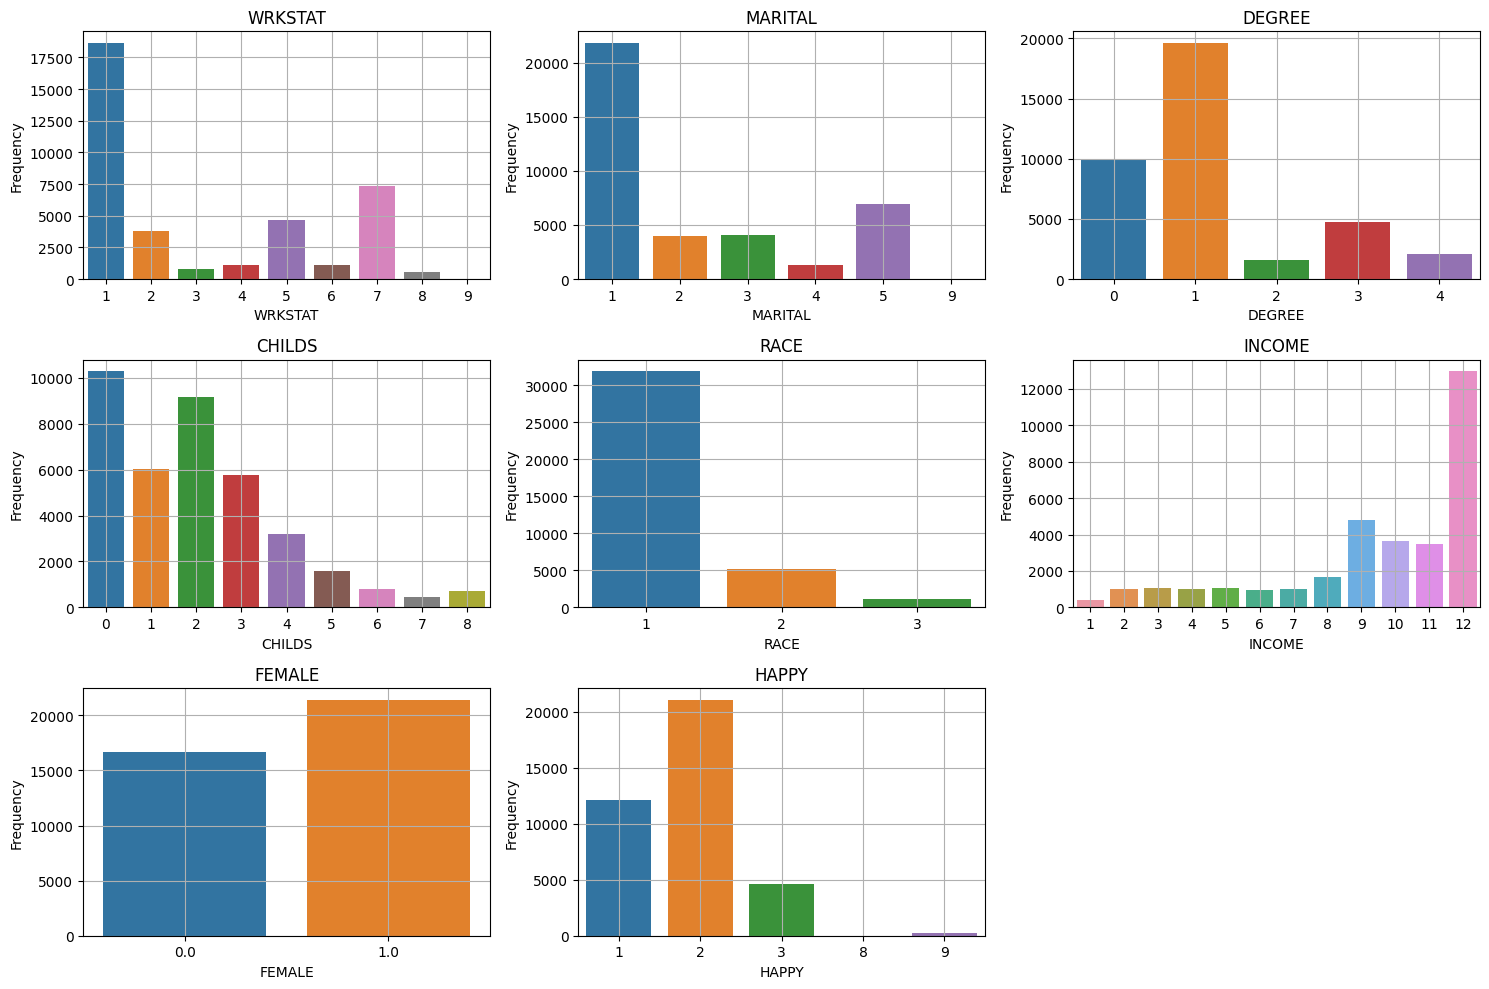
\includegraphics[width=0.6\linewidth]{figures/overall_frequency.png}
        \caption{Biểu đồ tần suất các giá trị của các trường dữ liệu được tính trên toàn tập dữ liệu}
        \label{fig:overall_frequency}
    \end{figure}

    Hình \ref{fig:overall_frequency} biểu diễn biểu đồ tần suất các giá trị của các trường dữ liệu.
    Trường WRKSTAT giá trị số 1 có số lượng xuất hiện nhiều nhất.
    Trường DEGREE giá trị số 1 có số lượng xuất hiện nhiều nhất.
    Đa số những người có số con từ 0 đến 3 con.
    Trường INCOME đa số mọi người đang ở trạng thái giá trị 12.

    \begin{figure}[H]
        \centering
        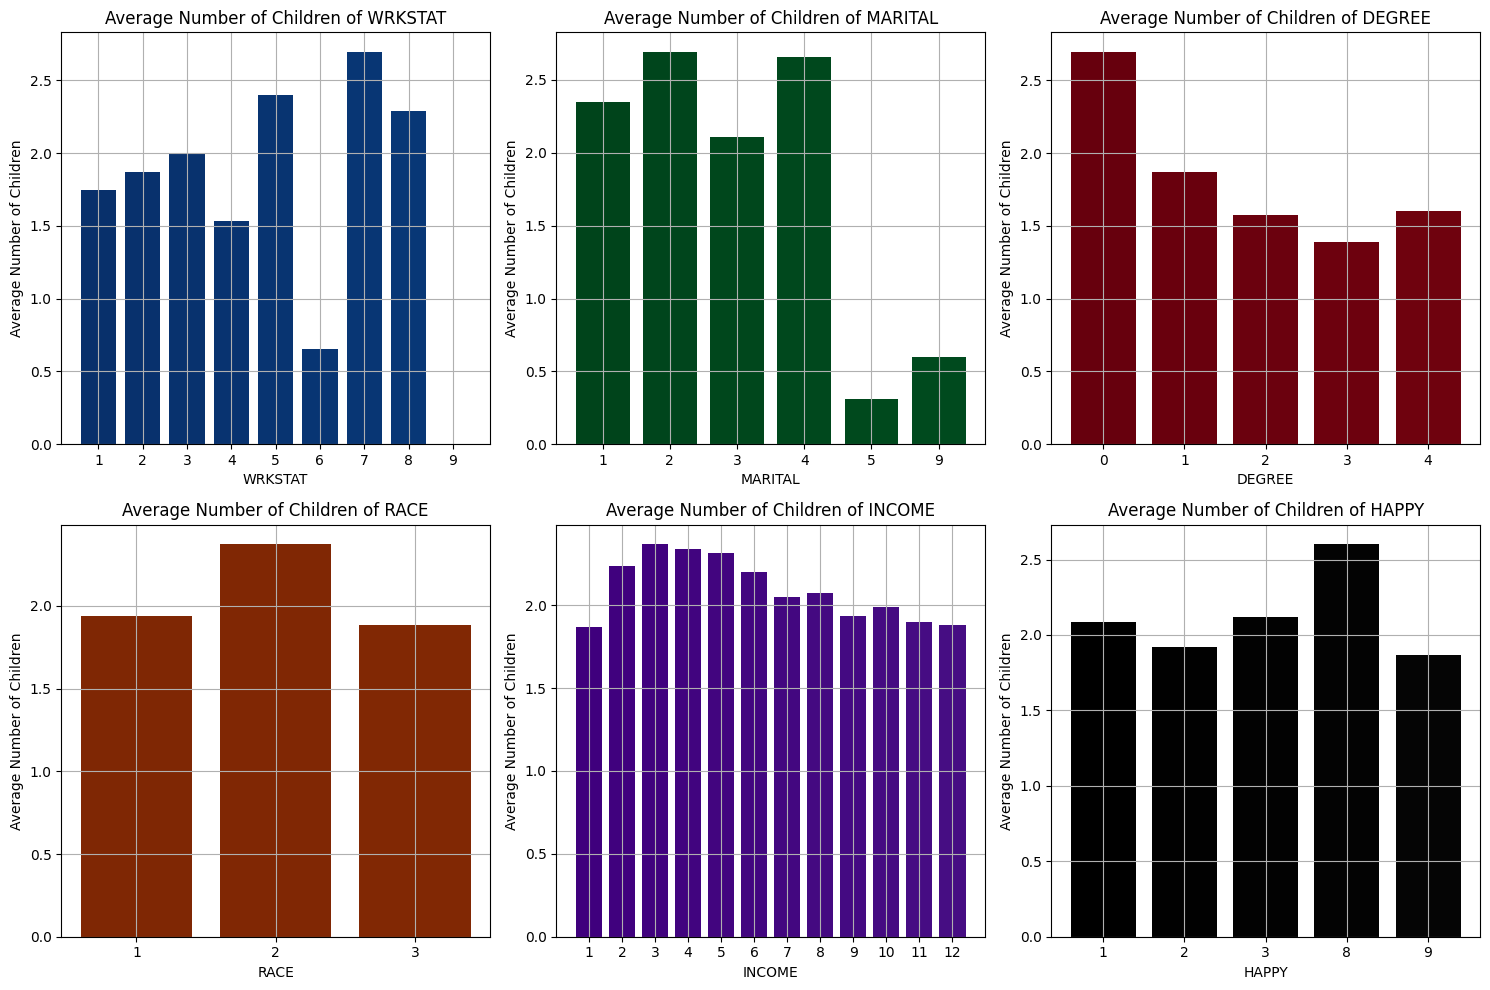
\includegraphics[width=0.7\linewidth]{figures/overall_avg_child_field.png}
        \caption{Biểu đồ cột với trục hoành là giá trị của các trường và trục tung là số lượng trẻ em sinh trung bình của những người tham gia khảo sát có giá trị tương ứng trong trường được tính trên toàn tập dữ liệu}
        \label{fig:overall_avg_child_field}
    \end{figure}

    Hình \ref{fig:overall_avg_child_field} biểu diễn số lượng trẻ em sinh trung bình của những người tham gia khảo sát có giá trị tương ứng trong trường được tính trên toàn tập dữ liệu.
    Với trường DEGREE ta nhận thấy chỉ số càng thấp thì số lượng trẻ em sinh trung bình càng cao.
    Trường INCOME, ở khu vực chỉ số thấp số lượng trẻ em sinh trung bình từ một người tham gia có xu hướng cao hơn ở khu vực chỉ số cao.
    Trường RACE, chỉ số 2 có số lượng trẻ em sinh trung bình cao hơn so với hai chỉ số giá trị còn lại.
    Trường WRKSTAT, các chỉ số 5,7 và 8 có số lượng trẻ sinh trung bình cao hơn các chỉ số giá trị còn lại

    \begin{figure}[H]
        \centering
        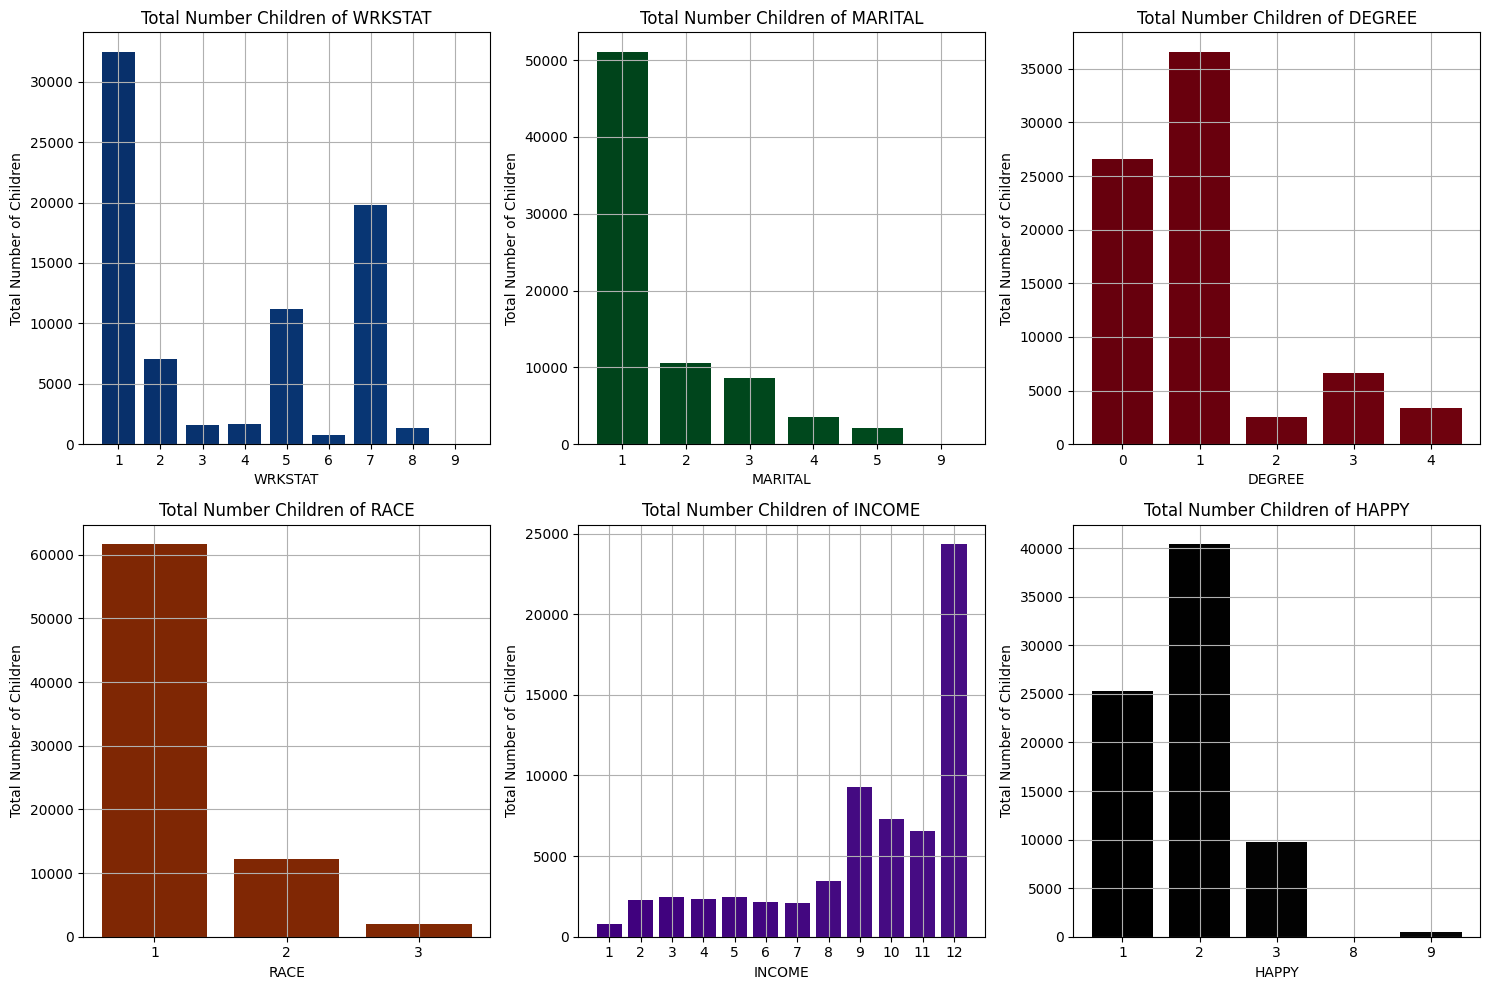
\includegraphics[width=0.7\linewidth]{figures/overall_total_child_field.png}
        \caption{Biểu đồ cột với trục hoành là giá trị của các trường và trục tung là tổng số lượng trẻ em được sinh của những người tham gia khảo sát có giá trị tương ứng trong trường được tính trên toàn tập dữ liệu}
        \label{fig:overall_total_child_field}
    \end{figure}

    Hình \ref{fig:overall_total_child_field} biểu diễn tổng số lượng trẻ em được sinh của những người tham gia khảo sát có giá trị tương ứng trong trường được tính trên toàn tập dữ liệu.
    Ta nhận thấy chủ yếu số lượng trẻ em được sinh ra khi bố mẹ đang ở trạng thái WRKSTAT là 1, MARITAL trạng thái là 1, RACE là 1, INCOME ở trạng thái 12, HAPPY chỉ số là 2.

    \begin{figure}[H]
        \centering
        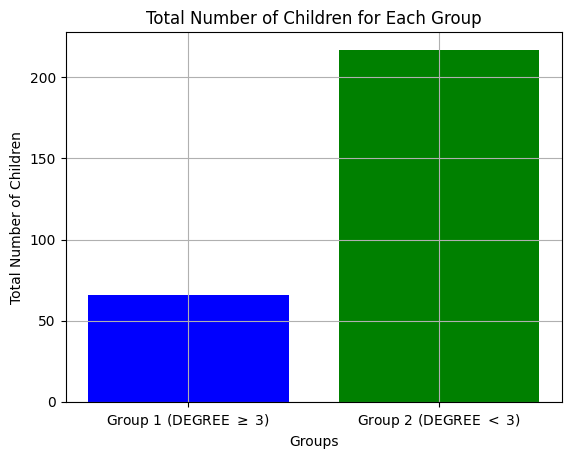
\includegraphics[width=0.5\linewidth]{figures/considered_total_child_each_women_group.png}
        \caption{Tổng số trẻ em được sinh ra từ hai nhóm phụ nữ, nhóm 1 có trình độ văn hóa trên phổ thông (DEG $\geq$ 3), nhóm 2 có trình độ văn hóa còn lại (DEG $<$ 3), số liệu được tính sau khi dữ liệu đã được lọc theo yêu cầu của đề bài}
        \label{fig:considered_total_child_each_women_group}
    \end{figure}

    Hình \ref{fig:considered_total_child_each_women_group} biểu diễn tổng số trẻ em sinh ra từ hai nhóm phụ nữ, nhóm 1 có trình độ văn hóa trên phổ thông (DEG $\geq$ 3), nhóm 2 có trình độ văn hóa còn lại (DEG $<$ 3), số liệu được tính sau khi dữ liệu đã được lọc theo yêu cầu của đề bài.
    Sau khi lọc, tổng số phụ nữ là đối tượng quan tâm là 156.
    Nhưng 1 quan sát có trường DEGREE là null.
    Số phụ nữ thuộc nhóm 1 là nhóm phụ nữ có trình độ văn hóa trên phổ thông (DEG $\geq$ 3) là 44.
    Tổng số trẻ em được nhóm phụ nữ số 1 sinh ra là 66.
    Số phụ nữ thuộc nhóm 2 là nhóm phụ nữ có trình độ văn hóa còn lại (DEG $<$ 3) là 111.
    Tổng số trẻ em được nhóm phụ nữ số 2 sinh ra là 217.

    \begin{figure}[H]
        \centering
        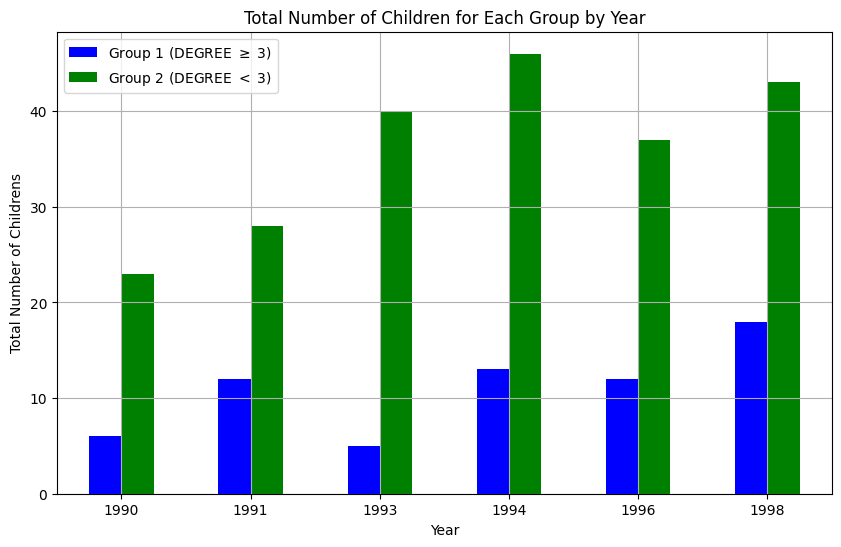
\includegraphics[width=0.8\linewidth]{figures/considered_total_child_each_women_group_each_year.png}
        \caption{Số lượng trẻ em sinh ra được sinh ra từ hai nhóm phụ nữ trong từng năm trong các năm 1990, 1991, 1993, 1994, 1996, 1998 trong dữ liệu đã được lọc}
        \label{fig:considered_total_child_each_women_group_each_year}
    \end{figure}

    Hình \ref{fig:considered_total_child_each_women_group_each_year} thể hiện số lượng trẻ em sinh ra được sinh ra từ hai nhóm phụ nữ trong từng năm trong các năm 1990, 1991, 1993, 1994, 1996, 1998 trong dữ liệu đã được lọc.
    Ta nhận thấy số lượng trẻ em do những phụ nữ thuộc nhóm 2 sinh ra luôn cao hơn số lượng trẻ em do những phụ nữ thuộc nhóm 1 sinh ra trong từng năm.
    Và qua các năm, số lượng trẻ em được sinh ra do cả hai nhóm phụ nữ có xu hướng tăng lên.

    \begin{figure}[H]
        \centering
        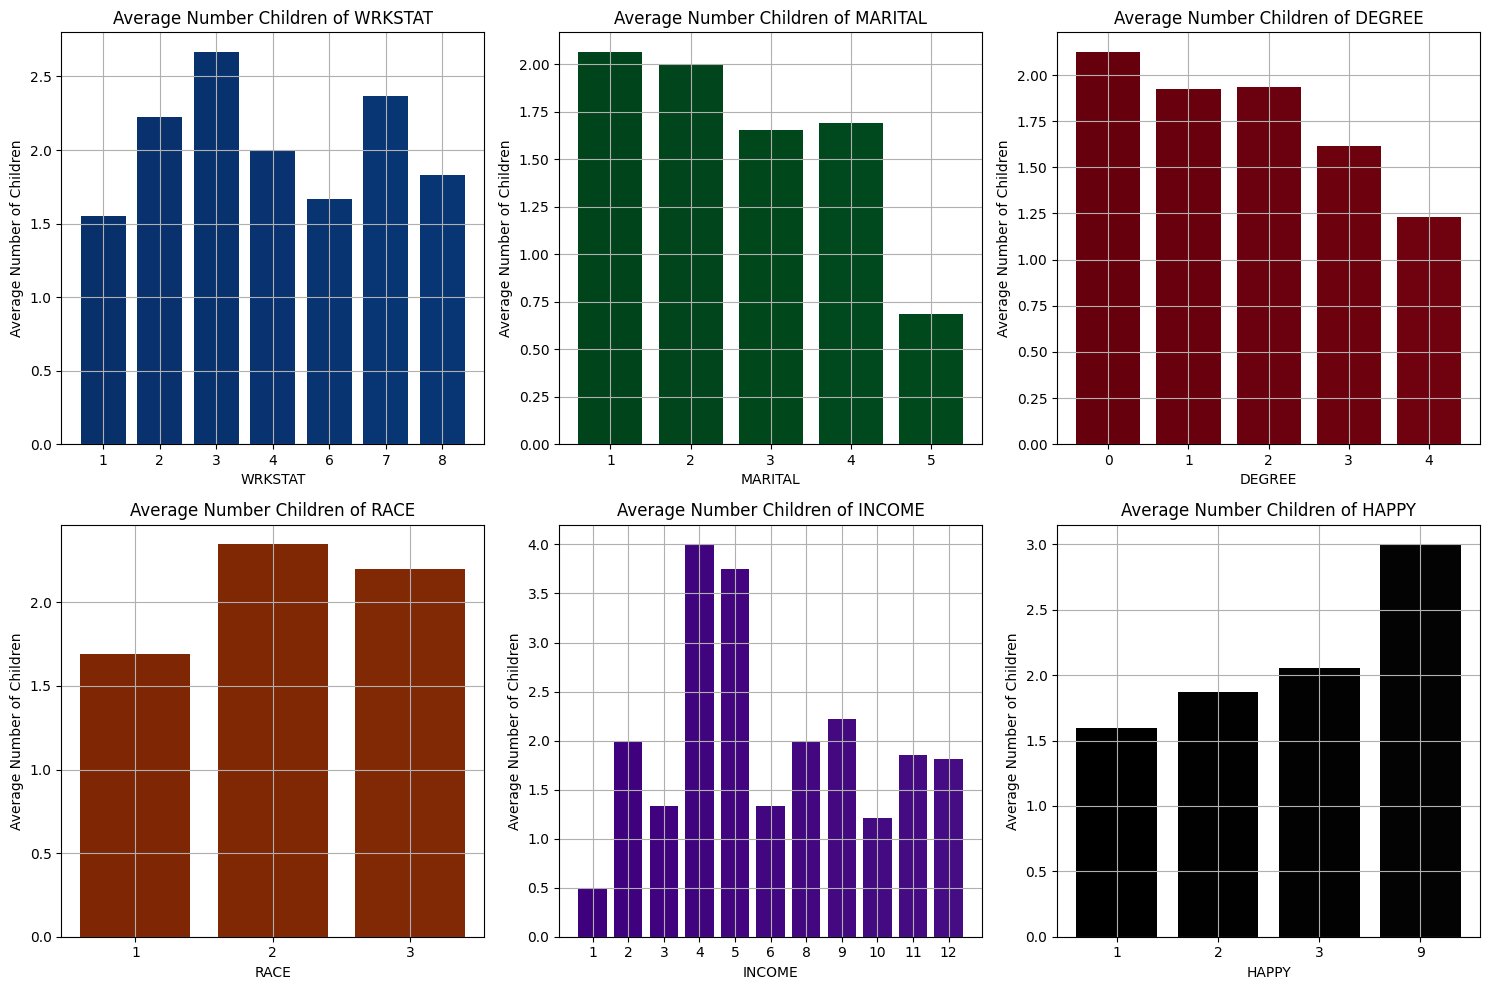
\includegraphics[width=0.8\linewidth]{figures/considered_avg_child_field.png}
        \caption{Số lượng trẻ em trung bình được sinh ra từ nhóm phụ nữ tương ứng với giá trị của từng trường trong dữ liệu đã được lọc}
        \label{fig:considered_avg_child_field}
    \end{figure}

    Hình \ref{fig:considered_avg_child_field} biểu diễn số lượng trẻ em trung bình được sinh ra từ nhóm phụ nữ tương ứng với giá trị của từng trường trong dữ liệu đã được lọc.
    Ta nhận thấy trường WRKSTAT những phụ nữ có giá trị 2, 3 hoặc 7 có số trẻ em trung bình được sinh cao hơn các giá trị khác.
    Trường DEGREE cho thấy trình độ văn hóa càng cao thì số lượng trẻ em trung bình được sinh ra có xu hướng giảm.
    Trường RACE có giá trị 2 cho số lượng trẻ em trung bình được sinh ra cao nhân.
    Trường INCOME những phụ nữ có giá trị thuộc nhóm 4, 5 cho số trẻ em trung bình được sinh ra là cao nhất.
    Trường HAPPY, chỉ số càng cao thì số trẻ em trung bình được sinh ra có xu hướng càng tăng.

    \begin{figure}[H]
        \centering
        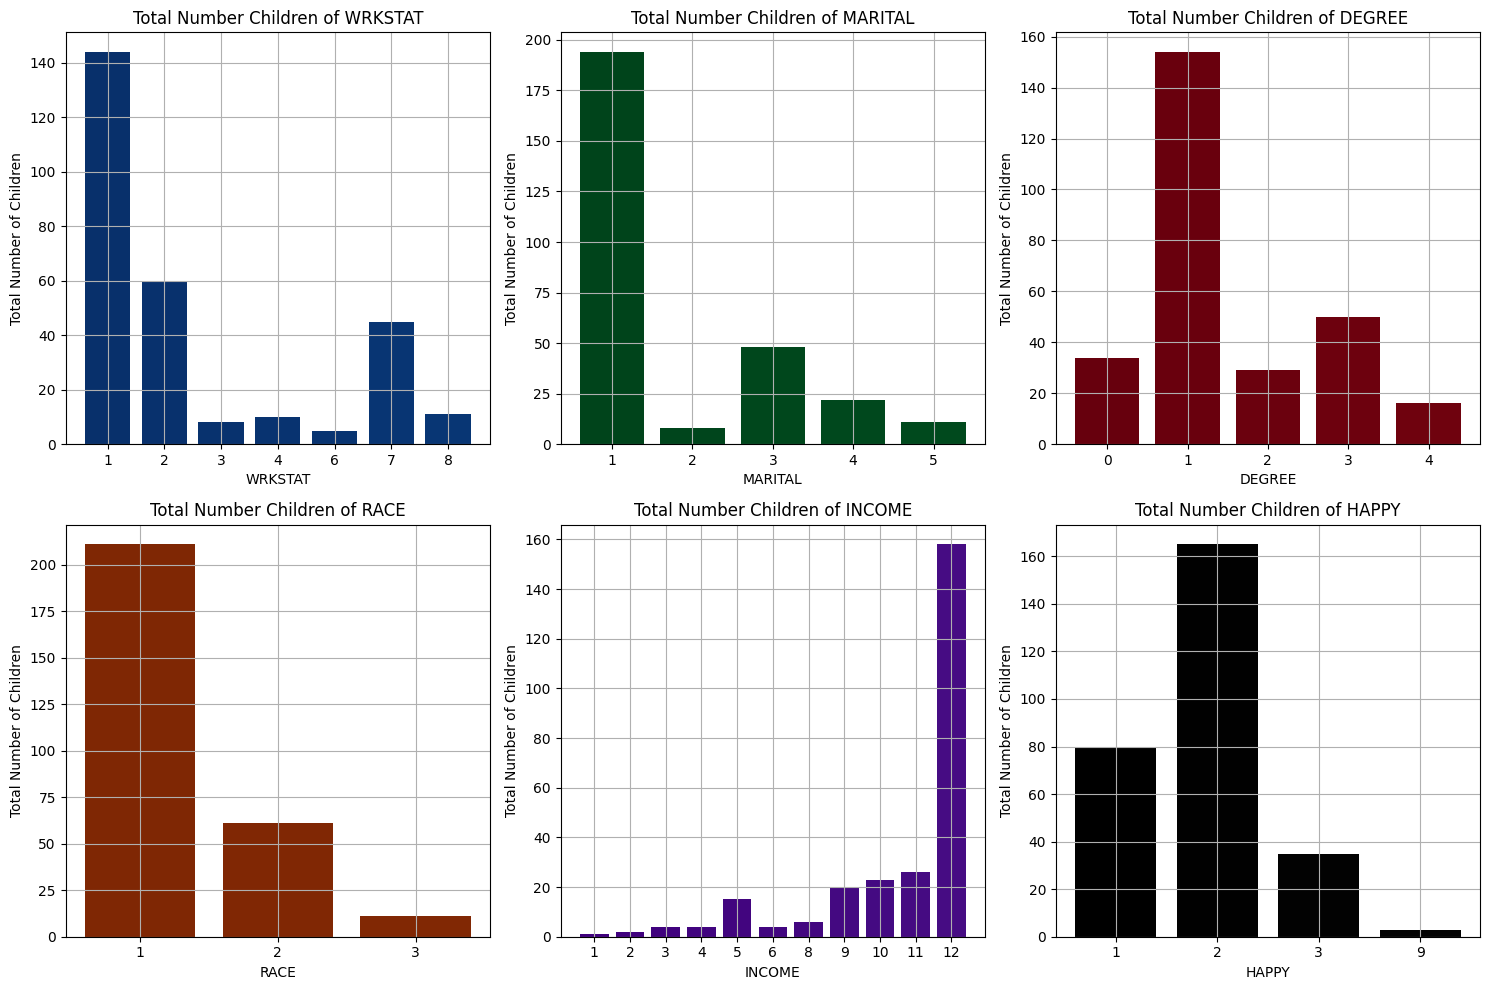
\includegraphics[width=0.8\linewidth]{figures/considered_total_child_field.png}
        \caption{Tổng số lượng trẻ em được sinh ra từ nhóm phụ nữ tương ứng với giá trị của từng trường trong dữ liệu đã được lọc}
        \label{fig:considered_total_child_field}
    \end{figure}

    Hình \ref{fig:considered_total_child_field} thể hiện tổng số lượng trẻ em được sinh ra từ nhóm phụ nữ tương ứng với giá trị của từng trường trong dữ liệu đã được lọc.
    Trường WRKSTAT những phụ nữ thuộc nhóm có giá trị 1 hoặc 2 đóng góp tổng số trẻ được sinh ra là lớn nhất.
    Trường MARITAL những phụ nữ thuộc nhóm có giá trị 1 sinh ra số lượng trẻ lớn hơn vượt trội so với nhóm còn lại.
    Trường DEGREE, số lượng trẻ được sinh bởi nhóm phụ nữ có giá trị 1 là lớn nhất.
    Đa số trẻ em được sinh ra từ phụ nữ có giá trị trường RACE là 1.
    Trường INCOME, những phụ nữ thuộc nhóm có giá trị 12 sinh ra số lượng trẻ lớn hơn tất cả các nhóm giá trị còn lại.
    Đa số trẻ em được sinh ra bởi những phụ nữ có giá trị HAPPY là 1 hoặc 2.

    Từ các phân tích trên, ta rút ra một số kết luận:

    \begin{itemize}
        \item Những phụ nữ thuộc nhóm RACE có giá trị 2 có số lượng trẻ em trung bình được sinh ra bởi một người phụ nữ là cao nhất.
        \item Khi giá trị trường DEGREE tăng thì số lượng trẻ em trung bình được sinh ra có xu hướng giảm.
        \item Đa số trẻ em được sinh ra từ những phụ nữ có trạng thái MARITAL là 1.
    \end{itemize}

    \textbf{2. Phần trả lời các câu hỏi ở trong bài tập ước lượng tham số Bayes cho tham số của phân phối Poisson:}

    \begin{enumerate}
        \item Xác định phân phối của dữ liệu (likelihood):
        
        Ta biết số lượng con sinh ra tuân theo phân phối Poisson.
        Ta gọi $X_i$ là số con sinh ra của một người phụ nữ thứ $i$ trong tập dữ liệu.
        Ta gọi tỷ lệ sinh là $\lambda$.
        Do $X \sim P(\lambda)$ nên:

        \begin{equation*}
            f(X=k \vert \lambda) = e^{-\lambda} \dfrac{\lambda^k}{k!}
        \end{equation*}

        Ta giả định số con được sinh từ một người phụ nữ là độc lập (các biến $X_i, i=1,2,\dots,n$ là các biến ngẫu nhiên độc lập và cùng tuân theo phân phối Poisson), và $x_i, i=1, 2, \dots, n$ là các giá trị quan sát tương ứng với $X_i, i=1, 2, \dots, n$:

        \begin{equation*}
            f(X_1=x_1,X_2=x_2,\dots, X_n=x_n \vert \lambda) = \prod_{i=1}^n f(X_i = x_i \vert \lambda)
        \end{equation*}

        với $n$ là số quan sát trong tập dữ liệu.

        Vậy phân phối của dữ liệu là:

        \begin{equation*}
            \begin{aligned}
                f(X_1=x_1,X_2=x_2,\dots, X_n=x_n \vert \lambda) &= \prod_{i=1}^n f(X_i = x_i \vert \lambda) \\
                &= \prod_{i=1}^n e^{-\lambda} \dfrac{\lambda^{x_1}}{x_1!} \\
                &= e^{-n\lambda} \dfrac{\lambda^{x_1 + x_2 + \dots + x_n}}{x_1! x_2! \dots x_n!} \\
                &= e^{-n\lambda} \dfrac{\lambda^{\sum_{i=1}^n x_i}}{\prod_{i=1}^n x_i!}
            \end{aligned}
        \end{equation*}

        \item Xác định phân phối hậu nghiệm của tỷ lệ sinh khi phân phối tiên nghiệm là:

        Ta gọi $g(\lambda)$ là phân phối tiên nghiệm của $\lambda$.
        Phân phối hậu nghiệm được tính bởi công thức:

        \begin{equation*}
            g(\lambda \vert X_1 =x_1, X_2=x_2, \dots, X_n=x_n) = \dfrac{g(\lambda) f(X_1=x_1,X_2=x_2,\dots, X_n=x_n \vert \lambda)}{\int g(\lambda) f(X_1=x_1,X_2=x_2,\dots, X_n=x_n \vert \lambda) d \lambda}
        \end{equation*}

        \textbf{Ta tìm phân phối hậu nghiệm của tỷ lệ sinh bằng lý thuyết:}

        \begin{enumerate}[label=(\alph*)]
            \item Phân phối đều
            
            Ta giả sử phân phối tiên nghiệm của $\lambda$ là:

            \begin{equation*}
                g(\lambda) = \begin{cases}
                    \dfrac{1}{a} \text{ nếu } \lambda \in \lbrack 0; a\rbrack (a > 0, a < \infty) \\
                    0 \text{ nếu ngược lại}
                \end{cases}
            \end{equation*}

            Như vậy ta có phân phối hậu nghiệm $g(\lambda \vert X_1 =x_1, X_2=x_2, \dots, X_n=x_n)$ của $\lambda$ là:

            \begin{equation*}
                \begin{aligned}
                    g(\lambda \vert X_1 =x_1, X_2=x_2, \dots, X_n=x_n) &= \dfrac{g(\lambda) f(X_1=x_1,X_2=x_2,\dots, X_n=x_n \vert \lambda)}{\int g(\lambda) f(X_1=x_1,X_2=x_2,\dots, X_n=x_n \vert \lambda) d \lambda} \\
                    &= \dfrac{\dfrac{1}{a} e^{-n\lambda} \dfrac{\lambda^{\sum_{i=1}^n x_i}}{\prod_{i=1}^n x_i!}}{\displaystyle\int_{0}^{a} \dfrac{1}{a} e^{-n\lambda} \dfrac{\lambda^{\sum_{i=1}^n x_i}}{\prod_{i=1}^n x_i!} d \lambda} \\
                    &= \dfrac{\dfrac{1}{a} e^{-n \lambda} \dfrac{(n\lambda)^{\sum_{i=1}^n x_i}}{\big(n^{\sum_{i=1}^n x_i}\big)\prod_{i=1}^n x_i!}}{\displaystyle\int_{0}^{a} \dfrac{1}{a} e^{-n\lambda} \dfrac{\lambda^{\sum_{i=1}^n x_i}}{\prod_{i=1}^n x_i!} d \lambda} \\
                    &= \dfrac{\dfrac{1}{a. n^{(\sum_{i=1}^n x_i) + 1}\prod_{i=1}^n x_i !}  ne^{-n\lambda} (n\lambda)^{\sum_{i=1}^n x_i}}{\dfrac{1}{a \prod_{i=1}^n x_i!} \displaystyle \int_{0}^a e^{-n\lambda}\lambda^{\sum_{i=1}^n x_i}d\lambda} \\
                    &= \dfrac{n e^{-n\lambda}(n\lambda)^{\sum_{i=1}^n x_i}}{n^{(\sum_{i=1}^n x_i) + 1}\displaystyle\int_{0}^a e^{-n\lambda} \lambda^{\sum_{i=1}^n x_i}d\lambda}
                \end{aligned}
            \end{equation*}

            Khi $a$ là hữu hạn, phân phối hậu nghiệm của tỷ lệ sinh sẽ không phụ thuộc vào $a$.
            Tổng quát, phân phối tiên nghiệm có thể có dạng:


            \begin{equation*}
                g(\lambda) = \begin{cases}
                    \dfrac{1}{d - c} \text{ nếu } \lambda \in \lbrack c; d\rbrack (d-c \text{ hữu hạn}) \\
                    0 \text{ nếu ngược lại}
                \end{cases}
            \end{equation*}

            Ta nhận thấy các đại lượng $a$ (theo giả thiết về phân phối tiên nghiệm), $n^{\sum_{i=1}^n x_i}$  (tập dữ liệu ta đã biết), $\displaystyle\int_{0}^a e^{-n\lambda} \lambda^{\sum_{i=1}^n x_i}d\lambda$ đều là hằng số.
            Nên phân phối hậu nghiệm $g(\lambda \vert X_1 =x_1, X_2=x_2, \dots, X_n=x_n)$ của $\lambda$ có dạng:

            \begin{equation*}
                \begin{aligned}
                    g(\lambda \vert X_1 =x_1, X_2=x_2, \dots, X_n=x_n) &= \dfrac{n e^{-n\lambda}(n\lambda)^{\sum_{i=1}^n x_i}}{n^{(\sum_{i=1}^n x_i) + 1}\displaystyle\int_{0}^a e^{-n\lambda} \lambda^{\sum_{i=1}^n x_i}d\lambda} \\
                    &= \dfrac{n e^{-n\lambda}(n\lambda)^{\big\lbrack(\sum_{i=1}^n x_i) + 1\big\rbrack - 1}}{\Gamma\big((\sum_{i=1}^n x_i) + 1\big)}.\dfrac{\Gamma\big((\sum_{i=1}^n x_i) + 1\big)}{n^{(\sum_{i=1}^n x_i) + 1}\displaystyle\int_{0}^a e^{-n\lambda} \lambda^{\sum_{i=1}^n x_i}d\lambda} \\
                    &\propto \dfrac{n e^{-n\lambda}(n\lambda)^{\big\lbrack(\sum_{i=1}^n x_i) + 1\big\rbrack - 1}}{\Gamma\big((\sum_{i=1}^n x_i) + 1\big)}
                \end{aligned}
            \end{equation*}

            với hàm $\Gamma(\alpha)$ được định nghĩa bằng:

            \begin{equation*}
                \Gamma(\alpha) = \int_{0}^{\infty} e^{-y} y^{\alpha - 1} dy
            \end{equation*}

            Ta chú ý phân phối hậu nghiệm của $\lambda$ nên $\lambda$ là biến.
            Mặt khác, ta có hàm mật độ xác suất của phân phối gamma (ta đặt biến ngẫu nhiên là $\lambda$ thay vì $x$ để dễ thấy sự tương tự giữa phân phối hậu nghiệm của $\lambda$ và phân phối gamma):

            \begin{equation*}
                \text{gamma}(\lambda; n, \alpha) = \begin{cases}
                    \dfrac{n e^{-n\lambda} (n\lambda)^{\alpha - 1}}{\Gamma(\alpha)} \text{ nếu } \lambda > 0 \\
                    0 \text{ nếu ngược lại}
                \end{cases}
            \end{equation*}

            Vì vậy:

            \begin{equation*}
                g(\lambda \vert X_1 =x_1, X_2=x_2, \dots, X_n=x_n) \propto \text{gamma}\big(\lambda; n, (\sum_{i=1}^n x_i) + 1\big)
            \end{equation*}

            \item Phân phối gamma
            
            Ta giả sử phân phối tiên nghiệm của $\lambda$ là:

            \begin{equation*}
                g(\lambda) = \text{gamma}(\lambda; r, \alpha) = \begin{cases}
                    \dfrac{r e^{-r\lambda} (r\lambda)^{\alpha - 1}}{\Gamma(\alpha)}=\dfrac{r^{\alpha}e^{-r\lambda} \lambda^{\alpha - 1}}{\Gamma(\alpha)} \text{ nếu } \lambda > 0 \\
                    0 \text{ nếu ngược lại}
                \end{cases}
            \end{equation*}

            Như vậy ta có phân phối hậu nghiệm $g(\lambda \vert X_1 =x_1, X_2=x_2, \dots, X_n=x_n)$ của $\lambda$ là:

            \begin{equation*}
                \begin{aligned}
                    &g(\lambda \vert X_1 =x_1, X_2=x_2, \dots, X_n=x_n) \\
                    &= \dfrac{g(\lambda) f(X_1=x_1,X_2=x_2,\dots, X_n=x_n \vert \lambda)}{\int g(\lambda) f(X_1=x_1,X_2=x_2,\dots, X_n=x_n \vert \lambda) d \lambda} \\
                    &= \dfrac{\dfrac{r^{\alpha}e^{-r\lambda} \lambda^{\alpha - 1}}{\Gamma(\alpha)} \dfrac{e^{-n\lambda} \lambda^{\sum_{i=1}^n x_i}}{\prod_{i=1}^n x_i!}}{\displaystyle \int_{0}^{\infty} \dfrac{r^{\alpha}e^{-r\lambda} \lambda^{\alpha - 1}}{\Gamma(\alpha)}  \dfrac{e^{-n\lambda}\lambda^{\sum_{i=1}^n x_i}}{\prod_{i=1}^n x_i!} d \lambda} \\
                    &= \dfrac{r^{\alpha}e^{-(n+r)\lambda} \lambda^{(\sum_{i=1}^n x_i) + \alpha - 1}}{\Gamma(\alpha)\prod_{i=1}^n x_i! \displaystyle \int_{0}^{\infty} \dfrac{r^{\alpha}e^{-r\lambda} \lambda^{\alpha - 1}}{\Gamma(\alpha)}  \dfrac{e^{-n\lambda}\lambda^{\sum_{i=1}^n x_i}}{\prod_{i=1}^n x_i!} d \lambda} \\
                    &= \dfrac{r^{\alpha}e^{-(n+r)\lambda} \lambda^{\sum_{i=1}^n x_i + \alpha - 1}}{\Gamma(\alpha)\prod_{i=1}^n x_i! \dfrac{r^{\alpha}}{\Gamma(\alpha)\prod_{i=1}^n x_i!} \displaystyle \int_{0}^{\infty} e^{-(n+r)\lambda} \lambda^{\sum_{i=1}^n x_i + \alpha - 1} d \lambda} \\
                    &= \dfrac{e^{-(n+r)\lambda} \lambda^{(\sum_{i=1}^n x_i) + \alpha - 1}}{\displaystyle \int_{0}^{\infty} e^{-(n+r)\lambda} \lambda^{(\sum_{i=1}^n x_i) + \alpha - 1} d \lambda} \\
                    &= \dfrac{(n+r)e^{-(n+r)\lambda}\lambda^{(\sum_{i=1}^n x_i) + \alpha - 1}}{(n+r)^{(\sum_{i=1}^n x_i) + \alpha} .\dfrac{1}{(n+r)^{(\sum_{i=1}^n x_i) + \alpha}}\displaystyle\int_{0}^{\infty}e^{-(n+r)\lambda}\lambda^{(\sum_{i=1}^n x_i) + \alpha - 1}d\lbrack (n+r)\lambda \rbrack} \\
                    &= \dfrac{(n+r)e^{-(n+r)\lambda}\lambda^{(\sum_{i=1}^n x_i) + \alpha - 1}}{\displaystyle\int_{0}^{\infty}e^{-(n+r)\lambda}\lambda^{(\sum_{i=1}^n x_i) + \alpha - 1}d\lbrack (n+r)\lambda \rbrack} \text{ (mẫu số chính là } \Gamma\big( (\sum_{i=1}^n x_i) + \alpha \big)) \\
                    &= \dfrac{(n+r)e^{-(n+r)\lambda}\lambda^{(\sum_{i=1}^n x_i) + \alpha - 1}}{\Gamma\big( (\sum_{i=1}^n x_i) + \alpha \big)} \\
                    &= \text{gamma}\big(\lambda; (n+r), (\sum_{i=1}^n x_i) + \alpha \big)
                \end{aligned}
            \end{equation*}

            Như vậy ta nhận thấy phân phối hậu nghiệm $g(\lambda \vert X_1 =x_1, X_2=x_2, \dots, X_n=x_n)$ của $\lambda$ cũng chính là phân phối gamma khi phân phối tiên nghiệm của $\lambda$ là phân phối gamma.
        \end{enumerate}

        \textbf{Sử dụng thực nghiệm để kiểm chứng các phân phối hậu nghiệm lý thuyết:}Để kiểm chứng các phân phối hậu nghiệm tìm được từ lý thuyết, ta sẽ sử dụng thực nghiệm để kiểm chứng các phân phối hậu nghiệm vừa tìm được.
        Do số lượng các điểm để tính giá trị của hàm mật độ xác suất tại các điểm này là lớn và số quan sát trong từng nhóm phụ nữ cũng lớn nên ta rất khó tính thủ công.
        Vì vậy ta sẽ sử dụng chương trình
        Ta sử dụng phương pháp lặp cho từng quan sát, ta lấy các điểm rời rạc, tính giá trị các điểm này theo hàm mật độ xác suất của phân phối tiên nghiệm đang xét.
        Do tổng giá trị của các điểm rời rạc phân phối tiên nghiệm phải là 1 nên sau khi tính giá trị các điểm này theo hàm mật độ xác suất, ta cần có bước chuẩn hóa bằng cách gán lại giá trị tại mỗi điểm bằng thương của giá trị tại mỗi điểm chia cho tổng giá trị tại các điểm.
        Cụ thể, ta chọn phân phối tiên nghiệm $g(\lambda)$.
        Ta chọn $m$ điểm $l_1, l_2, \dots, l_m$ trên trục hoành, ta tính giá trị các điểm này trên phân phối tiên nghiệm $g(e_1), g(e_2), \dots, g(e_m)$.
        Ta tính tiên nghiệm rời rạc bằng cách:

        \begin{equation*}
            \text{prior} = \Big \lbrack \dfrac{g(l_1)}{\sum_{i=1}^m g(l_i)}, \dfrac{g(l_2)}{\sum_{i=1}^m g(l_i)}, \dots, \dfrac{g(l_m)}{\sum_{i=1}^m g(l_i)} \Big \rbrack
        \end{equation*}

        Điều này đảm bảo tổng các điểm trên phân phối tiên nghiệm được rời rạc hóa là 1.
        Các giá trị này chỉ tỷ lệ mà không bằng chính xác với giá trị thật của các điểm trên phân phối tiên nghiệm liên tục.

        Để tính phân phối tiên nghiệm của tỷ lệ sinh sử dụng vòng lặp, mỗi vòng lặp ta tính hậu nghiệm cho từng quan sát, hậu nghiệm ở bước trước trở thành tiên nghiệm của vòng lặp sau (quan sát sau).
        Ta sử dụng mã giả sau để tính hậu nghiệm của một tập các quan sát tương ứng với một phân phối tiên nghiệm.


        \begin{algorithm}[h!]
            \DontPrintSemicolon
            \KwIn{Phân phối tiên nghiệm $g(\lambda)$, tập các quan sát $\lbrack x_1, x_2, \dots, x_n \rbrack$}
            \KwOut{Phân phối hậu nghiệm}
            Lấy một tập gồm m các điểm trên trục hoành $\lbrack l_1, l_2, \dots, l_m \rbrack$\;
            Tính giá trị các điểm này trên phân phối tiên nghiệm $\lbrack g(l_1), g(l_2), \dots, g(l_m) \rbrack$\;
            prior $\gets \Big \lbrack \dfrac{g(l_1)}{\sum_{k=1}^m g(l_i)}, \dfrac{g(l_2)}{\sum_{k=1}^m g(l_i)}, \dots, \dfrac{g(l_m)}{\sum_{k=1}^m g(l_i)} \Big \rbrack$\;
            \For{$i \gets 1$ \KwSty{to} $n$}{
                \For{$j \gets 1$ \KwSty{to} $m$} {
                    $pos_j \gets g(l_j) \times \dfrac{\exp(-l_j) \times l_j^{x_i}}{x_i!}$\;
                }
                posterior $\gets \Big \lbrack \dfrac{pos_1}{\sum_{k=1}^m pos_k}, \dfrac{pos_2}{\sum_{k=1}^m pos_k}, \dots, \dfrac{pos_m}{\sum_{k=1}^m pos_k} \Big \rbrack$\;
                prior $\gets$ posterior\;
            }
            \Return{posterior}\;
            \caption{Thủ tục tính phân phối hậu nghiệm tỷ lệ sinh sử dụng vòng lặp cho từng quan sát, hậu nghiệm ở bước trước trở thành tiên nghiệm của vòng lặp sau (quan sát sau).}
        \end{algorithm}

        Khi cài đặt chương trình, khi phân phối tiên nghiệm cho tỷ lệ sinh là phân phối gamma là $g(\lambda) = \text{gamma}(\lambda; r=2, \alpha=10)$, ta chọn $r=2, \alpha=10$.
        Ta sử đoạn chương trình sau:

        \begin{python}
lamdas = np.linspace(0, 10, 1000)

prior_uniform = np.ones_like(lamdas) / lamdas.shape[0]
            
r = 2
alpha = 10
            
prior_gamma = gamma_pdf_vector(lamdas, r, alpha)
prior_gamma = prior_gamma / np.sum(prior_gamma)
        \end{python}

        Đoạn code trên để chọn một tập các giá trị trên trục hoành, tính các giá trị tiên nghiệm trong trường hợp phân phối tiên nghiệm là phân phối đều và phân phối gamma.

        \begin{python}
plt.plot(lamdas, prior_gamma, label="gamma prior")
plt.xlabel("$\lambda$")
plt.legend()
plt.grid()
plt.show()
        \end{python}

        Đoạn code trên vẽ phân phối tiên nghiệm của tỷ lệ sinh là phân phối $g(\lambda)=\text{gamma}(\lambda;r=2,\alpha=10)$.

        \begin{figure}[h!]
            \centering
            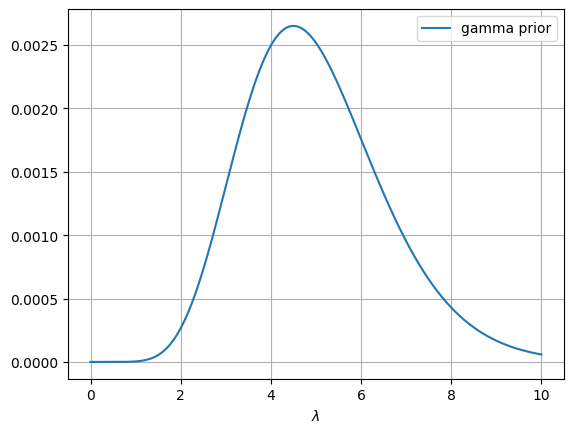
\includegraphics[width=0.6\linewidth]{figures/gamma_prior.png}
            \caption{Hình vẽ phân phối tiên nghiệm là phân phối gamma và đã được chuẩn hóa sao cho tổng giá trị các điểm là 1,
            các giá trị này chỉ tỷ lệ với giá trị thật trên hàm mật độ xác suất của phân phối gamma (do phải chuẩn hóa các điểm rời rạc)}
        \end{figure}

        \begin{python}
posterior_theory_uniform_deg_geq_3 = gamma_pdf_vector(lamdas, n_deg_geq_3, (child_total_deg_geq_3 + 1))
posterior_theory_uniform_deg_geq_3 = posterior_theory_uniform_deg_geq_3/np.sum(posterior_theory_uniform_deg_geq_3)
posterior_theory_gamma_deg_geq_3 = gamma_pdf_vector(lamdas, (n_deg_geq_3 + r), (child_total_deg_geq_3 + alpha))
posterior_theory_gamma_deg_geq_3 = posterior_theory_gamma_deg_geq_3/np.sum(posterior_theory_gamma_deg_geq_3)
        \end{python}

        Ta tính giá trị lý thuyết của phân phối hậu nghiệm tại các điểm trong trường hợp phân phối tiên nghiệm là phân phối đều và phân phối gamma cho nhóm phụ nữ có trình độ văn hóa trên phổ thông (DEG $\geq$ 3)

        \begin{python}
def compute_posterior_loop(prior: np.ndarray, lamdas: np.ndarray, observes: np.ndarray):
    poisson_vector = np.vectorize(poisson)
    for obs in tqdm(observes):
        numerator = prior * poisson_vector(x=obs, lamda=lamdas)
        pos = numerator / np.sum(numerator)
        prior = pos
            
    return pos
        \end{python}

        Hàm compute\_posterior\_loop thực hiện tính phân phối hậu nghiệm theo bước lặp các quan sát, ậu nghiệm của quan sát trước trở thành tiên nghiệm của quan sát sau

        \begin{python}
posterior_loop_uniform_deg_geq_3 = compute_posterior_loop(prior=prior_uniform, lamdas=lamdas, observes=df_deg_geq_3.CHILDS.to_numpy())
posterior_loop_gamma_deg_geq_3 = compute_posterior_loop(prior=prior_gamma, lamdas=lamdas, observes=df_deg_geq_3.CHILDS.to_numpy())
        \end{python}
        Ta tính giá trị của phân phối hậu nghiệm tại các điểm bằng (cho từng quan sát, hậu nghiệm ở bước trước trở thành tiên nghiệm ở bước sau) vòng lặp trong trường hợp phân phối tiên nghiệm là phân phối đều và phân phối gamma cho nhóm phụ nữ có trình độ văn hóa trên phổ thông (DEG $\geq$ 3)

        \begin{python}
def plot_posterior_comparison(lamdas, pos_theory, pos_loop, prior_type="uniform"):
    plt.plot(lamdas, pos_theory, label="posterior {} theory".format(prior_type), linestyle="dashed")
    plt.plot(lamdas, pos_loop, label="posterior loop", linestyle="dotted")
    plt.xlabel("$\lambda$")
    plt.grid()
    plt.legend()
    plt.show()
        \end{python}

        Hàm vẽ so sánh phân phối hậu nghiệm từ lý thuyết và phân phối hậu nghiệm từ vòng lặp (cho từng quan sát cho từng quan sát, hậu nghiệm ở bước trước trở thành tiên nghiệm ở bước sau)

        \begin{python}
plot_posterior_comparison(lamdas=lamdas, pos_theory=posterior_theory_uniform_deg_geq_3, pos_loop=posterior_loop_uniform_deg_geq_3, prior_type="uniform")
        \end{python}

        Ta vẽ so sánh phân phối hậu nghiệm được tính từ lý thuyết và vòng lặp khi phân phối tiên nghiệm là phân phối đều cho nhóm phụ nữ có trình độ văn hóa trên phổ thông (DEG $\geq$ 3)

        \begin{figure}[h!]
            \centering
            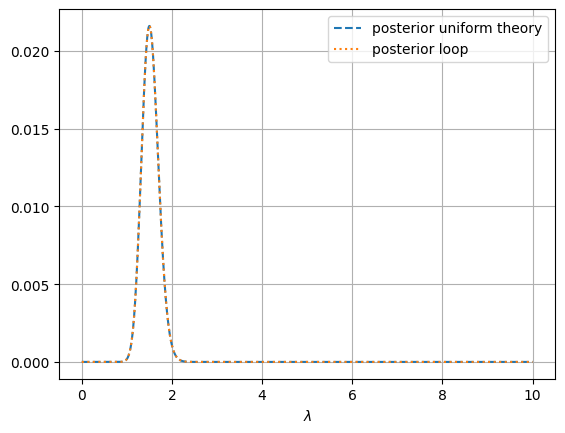
\includegraphics[width=0.6\linewidth]{figures/posterior_loop_theory_uniform_deg_geq_3.png}
            \caption{Phân phối hậu nghiệm được tính từ lý thuyết và vòng lặp khi phân phối tiên nghiệm là phân phối đều cho nhóm phụ nữ có trình độ văn hóa trên phổ thông (DEG $\geq$ 3)}
            \label{fig:posterior_loop_theory_uniform_deg_geq_3}
        \end{figure}

        \begin{python}
plot_posterior_comparison(lamdas=lamdas, pos_theory=posterior_theory_gamma_deg_geq_3, pos_loop=posterior_loop_gamma_deg_geq_3, prior_type="gamma")
        \end{python}

        Vẽ so sánh phân phối hậu nghiệm được tính từ lý thuyết và vòng lặp khi phân phối tiên nghiệm là phân phối gamma ($r=2$ và $\alpha=10$) cho nhóm phụ nữ có trình độ văn hóa trên phổ thông (DEG $\geq$ 3)

        \begin{figure}[h!]
            \centering
            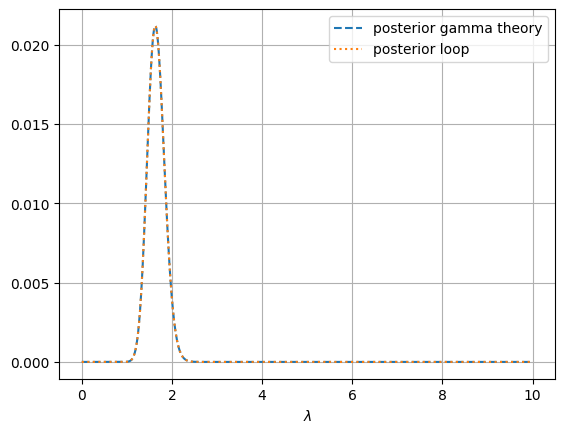
\includegraphics[width=0.6\linewidth]{figures/posterior_loop_theory_gamma_deg_geq_3.png}
            \caption{Phân phối hậu nghiệm được tính từ lý thuyết và vòng lặp khi phân phối tiên nghiệm là phân phối gamma ($r=2$ và $\alpha=10$) cho nhóm phụ nữ có trình độ văn hóa trên phổ thông (DEG $\geq$ 3)}
            \label{fig:posterior_loop_theory_gamma_deg_geq_3}
        \end{figure}

        Từ hình \ref{fig:posterior_loop_theory_uniform_deg_geq_3} và hình \ref{fig:posterior_loop_theory_gamma_deg_geq_3}, ta nhận thấy phân phối hậu nghiệm của tỷ lệ sinh được tính từ lý thuyết và được tính từ thực nghiệm của nhóm phụ nữ có trình độ văn hóa trên phổ thông (DEG $\geq$ 3) là gần như hoàn toàn trùng khớp.

        \begin{python}
posterior_theory_uniform_deg_less_3 = normal_pdf_vector(lamdas, ((child_total_deg_less_3 + 1)/n_deg_less_3), np.sqrt((child_total_deg_less_3 + 1)/(n_deg_less_3**2)))
posterior_theory_uniform_deg_less_3 = posterior_theory_uniform_deg_less_3/np.sum(posterior_theory_uniform_deg_less_3)
posterior_theory_gamma_deg_less_3 = normal_pdf_vector(lamdas, ((child_total_deg_less_3 + alpha)/(n_deg_less_3 + r)), np.sqrt((child_total_deg_less_3 + alpha)/((n_deg_less_3 + r)**2)))
posterior_theory_gamma_deg_less_3 = posterior_theory_gamma_deg_less_3/np.sum(posterior_theory_gamma_deg_less_3)
        \end{python}

        Ta tính phân phối hậu nghiệm lý thuyết khi phân phối tiên nghiệm cho tỷ lệ sinh là phân phối đều và phân phối tiên nghiệm cho tỷ lệ sinh là phân phối gamma cho nhóm phụ nữ có trình độ văn hóa còn lại (DEG $<$ 3) 

        \begin{python}
posterior_loop_uniform_deg_less_3 = compute_posterior_loop(prior=prior_uniform, lamdas=lamdas, observes=df_deg_less_3.CHILDS.to_numpy())
posterior_loop_gamma_deg_less_3 = compute_posterior_loop(prior=prior_gamma, lamdas=lamdas, observes=df_deg_less_3.CHILDS.to_numpy())
        \end{python}

        Ta tính giá trị của phân phối hậu nghiệm tại các điểm bằng vòng lặp (cho từng quan sát, hậu nghiệm ở bước trước trở thành tiên nghiệm ở bước sau) khi phân phối tiên nghiệm cho tỷ lệ sinh là phân phối đều và phân phối tiên nghiệm cho tỷ lệ sinh là phân phối gamma cho nhóm phụ nữ có trình độ văn hóa còn lại (DEG $<$ 3)

        \begin{python}
plot_posterior_comparison(lamdas=lamdas, pos_theory=posterior_theory_uniform_deg_less_3, pos_loop=posterior_loop_uniform_deg_less_3, prior_type="uniform")
        \end{python}

        Ta vẽ so sánh phân phối hậu nghiệm được tính từ lý thuyết và vòng lặp khi phân phối tiên nghiệm cho tỷ lệ sinh là phân phối đều cho nhóm phụ nữ có trình độ văn hóa còn lại (DEG $<$ 3)

        \begin{figure}[h!]
            \centering
            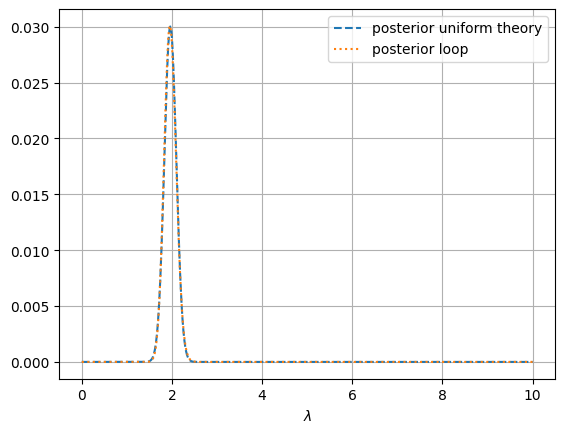
\includegraphics[width=0.6\linewidth]{figures/posterior_loop_theory_uniform_deg_less_3.png}
            \caption{Phân phối hậu nghiệm được tính từ lý thuyết và vòng lặp khi phân phối tiên nghiệm cho tỷ lệ sinh là phân phối đều cho nhóm phụ nữ có trình độ văn hóa còn lại (DEG $<$ 3)}
            \label{fig:posterior_loop_theory_uniform_deg_less_3}
        \end{figure}

        \begin{python}
plot_posterior_comparison(lamdas=lamdas, pos_theory=posterior_theory_gamma_deg_less_3, pos_loop=posterior_loop_gamma_deg_less_3, prior_type="gamma")
        \end{python}

        Vẽ so sánh phân phối hậu nghiệm được tính từ lý thuyết và vòng lặp khi phân phối tiên nghiệm là phân phối gamma ($r=2$ và $\alpha=10$) nhóm phụ nữ có trình độ văn hóa còn lại (DEG $<$ 3)

        \begin{figure}[h!]
            \centering
            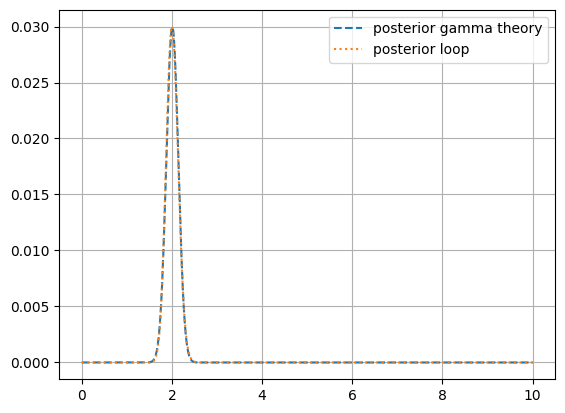
\includegraphics[width=0.6\linewidth]{figures/posterior_loop_theory_gamma_deg_less_3.png}
            \caption{Phân phối hậu nghiệm được tính từ lý thuyết và vòng lặp khi phân phối tiên nghiệm là phân phối gamma ($r=2$ và $\alpha=10$) nhóm phụ nữ có trình độ văn hóa còn lại (DEG $<$ 3)}
            \label{fig:posterior_loop_theory_gamma_deg_less_3}
        \end{figure}

        Từ hình \ref{fig:posterior_loop_theory_uniform_deg_less_3} và hình \ref{fig:posterior_loop_theory_gamma_deg_less_3}, ta nhận thấy phân phối hậu nghiệm của tỷ lệ sinh được tính từ lý thuyết và được tính từ thực nghiệm của nhóm phụ nữ có trình độ văn hóa còn lại (DEG $<$ 3) là gần như hoàn toàn trùng khớp.

        \textbf{Nhận xét:} Ta nhận thấy kết quả lý thuyết tìm được và kết quả nhận được từ thực nghiệm (sử dụng vòng lặp cho từng quan sát, hậu nghiệm ở bước trước trở thành tiên nghiệm ở bước sau) cho các phân phối của tỷ lệ sinh là trùng khớp với nhau.

        \item Đặc điểm của các phân phối hậu nghiệm tìm được là:
        
        Như ta đã chứng minh, khi phân phối tiên nghiệm là phân phối đều hoặc phân phối gamma thì phân phối hậu nghiệm đều có dạng phân phối gamma.

        Ta sẽ xét phân phối gamma $\text{gamma}(\lambda; r, \alpha)$ khi cả $r$ và $\alpha$ đều lớn.
        Ta sử dụng công cụ hàm sinh mômen.
        Cho một đại lượng ngẫu nhiên $Y$, khi đó nếu tồn tại $\mathbb{E}(e^{tY}), \forall \lvert t \rvert \leq k, k > 0$ bất kỳ.
        Ta gọi $M(t) = \mathbb{E}(e^{tY})$ là hàm sinh mômen của $Y$:

        Ta xét trường hợp $Z \sim \mathcal{N}(0; 1)$:

        \begin{equation*}
            \begin{aligned}
                M(t) &= \mathbb{E}(e^{tz}) \\
                &=\int_{-\infty}^{\infty} e^{tz} \dfrac{1}{\sqrt{2\pi}} e^{-\frac{z^2}{2}} dz \\
                &=\int_{-\infty}^{\infty} \dfrac{1}{\sqrt{2\pi}} e^{-\dfrac{(y^2-2ty)}{2}} dy \\
                &=\int_{-\infty}^{\infty} \dfrac{1}{\sqrt{2\pi}} e^{-\dfrac{(z-t)^2}{2}}e^{\dfrac{t^2}{2}} dz \\
                &=e^{\dfrac{t^2}{2}}\int_{-\infty}^{\infty} \underbrace{\dfrac{1}{\sqrt{2\pi}} e^{-\dfrac{(z-t)^2}{2}}}_{\mathcal{N}(t;1)} dz \\
                &=e^{\dfrac{t^2}{2}}\int_{-\infty}^{\infty} \mathcal{N}(t;1) dz \\
                &=e^{\dfrac{t^2}{2}}
            \end{aligned}
        \end{equation*}

        Ta xét với biến ngẫu nhiên $Y = aZ + b$, ta tìm hàm sinh mômen của $Z$ khi ta đã biến hàm sinh mômen của biến ngẫu nhiên $Y$:

        \begin{equation*}
            \begin{aligned}
                M_Y (t) &= \mathbb{E} (e^{tZ}) \\
                &= \mathbb{E} (e^{t(aZ + b)}) \\
                &= \mathbb{E} (e^{t(aZ + b)}) \\
                &= \mathbb{E} (e^{aZt}e^{bt}) \\
                &= e^{bt} \mathbb{E}(e^{aZt}) \\
                &= e^{bt} M_Z(at)
            \end{aligned}
        \end{equation*}

        Vậy với biến ngẫu nhiên $Y \sim \mathcal{\mu; \sigma^2}$, ta có thể viết biến ngẫu nhiên $Y$ dưới dạng: $Y = \mu + \sigma Z$ với $Z \sim \mathcal{N}(0;1)$ nên:

        \begin{equation*}
            \begin{aligned}
                M_Y(t) &= e^{\mu t} M_z(\sigma t) \\
                &= e^{\mu t} e^{\dfrac{\sigma^2 t^2}{2}} \\
                &= e^{\mu t + \dfrac{\sigma^2 t^2}{2}}
            \end{aligned}
        \end{equation*}

        Ta tìm hàm sinh mômen của phân phối gamma:

        \begin{equation*}
            \begin{aligned}
                M(t) &= \mathbb{E}(e^{t\lambda}) \\
                &= \int_{-\infty}^{\infty} e^{t\lambda} \dfrac{r^{\alpha}e^{-r\lambda} \lambda^{\alpha-1}}{\Gamma(\alpha)} d\lambda (t < r) \\
                &= \dfrac{r^{\alpha}}{\Gamma(\alpha)} \int_{-\infty}^{\infty} e^{-(r-t)\lambda} \lambda^{\alpha-1} d \lambda \\
                &= \dfrac{r^{\alpha}}{\Gamma(\alpha)} \int_{-\infty}^{\infty} \dfrac{1}{(r-t)^{\alpha}} e^{-(r-t)\lambda} ((r-t)\lambda)^{\alpha-1} d (r-t)\lambda \\
                &= \dfrac{r^{\alpha}}{\Gamma(\alpha)(r-t)^{\alpha}} \underbrace{\int_{-\infty}^{\infty} e^{-(r-t)\lambda} ((r-t)\lambda)^{\alpha-1} d (r-t)\lambda}_{\Gamma(\alpha)} \\
                &= \dfrac{r^{\alpha} \Gamma(\alpha)}{(r-t)^{\alpha}\Gamma(\alpha)} \\
                &= \dfrac{r^{\alpha}}{(r-t)^{\alpha}} \\
                &= \Big( \dfrac{r}{r-t} \Big)^{\alpha}
            \end{aligned}
        \end{equation*}

        \begin{dl} \label{dl:1}
            Cho biến ngẫu nhiên $Y$ có hàm sinh mômen là $M_Y(t)$. 
            Biến ngẫu nhiên $Z$ có hàm sinh mômen là $M_Z(t)$.
            Với một số $k > 0$ tùy ý, nếu $\forall \lvert t \rvert < k$ thỏa mãn:
            \begin{equation*}
                M_Y(t) = M_Z(t) \forall \lvert t \vert < k
            \end{equation*}
            thì $Y$ và $Z$ cùng phân phối.
        \end{dl}

        Đối với hàm sinh mômen, khi $t$ đủ nhỏ, $r$ và $\alpha$ khá lớn, hàm sinh mômen $\Big( \dfrac{r}{r-t} \Big)^{\alpha}$ sẽ có dạng $1^{\infty}$.
        Từ giới hạn cơ bản:

        \begin{equation*}
            \lim_{a \rightarrow 0} (1 + a)^{\frac{1}{a}} = e
        \end{equation*}
        Ta xét giới hạn:

        \begin{equation*} 
            \begin{aligned}
                \lim_{\begin{subarray}{l} t \rightarrow 0 \\ r \rightarrow \infty \end{subarray}} \Big( \dfrac{r}{r-t} \Big)^{\alpha} &= \lim_{\begin{subarray}{l} t \rightarrow 0 \\ r \rightarrow \infty \end{subarray}} \Big( \dfrac{r-t + t}{r-t} \Big)^{\alpha} \\
                &= \lim_{\begin{subarray}{l} t \rightarrow 0 \\ r \rightarrow \infty \end{subarray}} \Big(1 + \dfrac{t}{r-t} \Big)^{\alpha} \\
                &= \lim_{\begin{subarray}{l} t \rightarrow 0 \\ r \rightarrow \infty \end{subarray}} \Big(1 + \dfrac{t}{r-t} \Big)^{\dfrac{r-t}{t} \dfrac{\alpha t}{r-t}} \\
                &= \exp\Big(\dfrac{\alpha t}{r-t} \Big) \\
                &= \exp\Bigg(\dfrac{\alpha t}{r(1 - \dfrac{t}{r})} \Bigg)
            \end{aligned}
        \end{equation*}

        Ta sử dụng khai triển Maclaurin phần dư dạng Peano:
        \begin{equation*}
            \dfrac{1}{1-a} = 1 + a + a^2 + a^3 + \dots + a^n + o(a^n), \text{ miền hội tụ } \lvert a \rvert < 1
        \end{equation*}

        Như vậy:

        \begin{equation*}
            \begin{aligned}
                \exp\Bigg(\dfrac{\alpha t}{r(1 - \dfrac{t}{r})} \Bigg) &= \exp\Bigg(\dfrac{\alpha t}{r}(1 + \dfrac{t}{r} + \dfrac{t^2}{r^2} + o(t^2)) \Bigg) \\
                &\approx \exp\Bigg( \dfrac{\alpha t}{r} + \dfrac{\alpha t^2}{r^2}\Bigg)
            \end{aligned}
        \end{equation*}

        Ta nhận thấy $\exp\Bigg( \dfrac{\alpha t}{r} + \dfrac{\alpha t^2}{r^2}\Bigg)$ chính là hàm sinh mômen của phân phối chuẩn $\mathcal{N}\Big(\dfrac{\alpha}{r}; \dfrac{\alpha}{r^2} \Big)$.
        Khi $k > 0$ đủ nhỏ $\forall \lvert t \rvert <k$ và $r$ đủ lớn sao cho hàm sinh mômen của phân phối gamma xấp xỉ bằng hàm sinh mômen của phân phối chuẩn, theo định lý \ref{dl:1}:

        \begin{equation*}
            \text{gamma}(\lambda; r, \alpha) \approx \mathcal{N}\Big(\dfrac{\alpha}{r};\dfrac{\alpha}{r^2}\Big)
        \end{equation*}

        Để kiểm chứng kết quả lý thuyết trên, ta sẽ vẽ phân phối $\text{gamma}(\lambda; 30, 90) (r=30, \alpha=90)$ và phân phối chuẩn $\mathcal{N}\Big(\dfrac{\alpha}{r}=\dfrac{90}{30}=3, \dfrac{\alpha}{r^2}=\dfrac{1}{10}\Big)$ bằng đoạn code:

        \begin{python}
def gamma_pdf(x, r: float, alpha: float):
    return (r**alpha * np.exp(-r*x) * x**(alpha - 1)) / gamma(alpha)


def normal_pdf(x, mu: float, sigma: float):
    return ((1/(sigma * np.sqrt(2*np.pi))) * np.exp(-((x-mu)**2/(2*sigma**2))))

gamma_pdf_vector = np.vectorize(gamma_pdf)
normal_pdf_vector = np.vectorize(normal_pdf)
x = np.linspace(0, 6, 1000)
gamma_distribution = gamma_pdf_vector(x, 30, 90)
normal_approx_of_gamma_distribution = normal_pdf_vector(x, 90/30, np.sqrt(90/(30**2)))
            
plt.plot(x, gamma_distribution, label="gamma distribution", linestyle="solid")
plt.plot(x, normal_approx_of_gamma_distribution, label="normal approximation of gamma distribution", linestyle="dashed")
plt.xlabel("$\lambda$")
plt.legend()
plt.grid()
plt.show()
        \end{python}

        \begin{figure}[h]
            \centering
            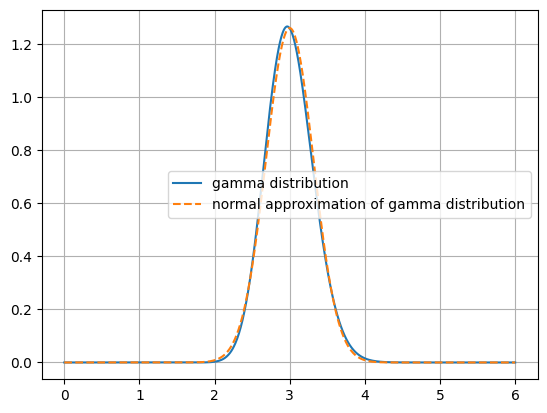
\includegraphics[width=0.6\linewidth]{figures/gamma_normal_approximation.png}
            \caption{Minh họa phân phối gamma xấp xỉ phân phối chuẩn khi hai tham số $r$ và $\alpha$ lớn}
            \label{fig:gamma_normal_approximation}
        \end{figure}
        Hình \ref{fig:gamma_normal_approximation} cho ta thấy phân phối gamma $\text{gamma}(\lambda; 30, 90)$ khi $r=30, \alpha=90$ xấp xỉ phân phối chuẩn $\mathcal{N}\Big(3, \dfrac{1}{10}\Big)$.
        Đỉnh (mode) của phân phối gamma nằm bên trái một chút so với phân phối chuẩn.
        Do đối với phân phối chuẩn trung bình và mode bằng nhau và bằng $\dfrac{\alpha}{r}$ còn đối với phân phối gamma mode bằng $\dfrac{\alpha - 1}{r}$.

        \item Ước lượng tỷ lệ sinh của 02 nhóm phụ nữ
        
        \textbf{Ước lượng điểm:}
        
        Để ước lượng tỷ lệ sinh của hai nhóm phụ nữ.
        Ta có thể sử dụng lấy trung bình hoặc mode của phân phối hậu nghiệm của tỷ lệ sinh của hai nhóm tương ứng.
        Đầu tiên ta sẽ tìm trung bình và mode từ phân phối hậu nghiệm lý thuyết của tỷ lệ sinh khi phân phối tiên nghiệm là phân phối đều hoặc phân phối tiên nghiệm là phân phối gamma
        Ta gọi $\hat{\lambda}$ là ước lượng của $\lambda$
        \begin{itemize}
            \item Phân phối tiên nghiệm là phân phối đều:
            
            Ta giả sử phân phối tiên nghiệm của $\lambda$ là:

            \begin{equation*}
                g(\lambda) = \begin{cases}
                    \dfrac{1}{a} \text{ nếu } \lambda \in \lbrack 0; a\rbrack (a > 0) \\
                    0 \text{ nếu ngược lại}
                \end{cases}
            \end{equation*}

            Ở câu 2, ta đã biết phân phối hậu nghiệm $g(\lambda \vert X_1 =x_1, X_2=x_2, \dots, X_n=x_n)$ có dạng phân phối gamma:

            \begin{equation*}
                g(\lambda \vert X_1 =x_1, X_2=x_2, \dots, X_n=x_n) \propto \text{gamma}\big(\lambda; n, (\sum_{i=1}^n x_i) + 1\big)
            \end{equation*}

            Nếu $\hat{\lambda}$ được tính theo trung bình của phân phối hậu nghiệm,
            ta gọi ước lượng này là $\hat{\lambda}_1$:

            \begin{equation*}
                \hat{\lambda}_1 = \dfrac{(\sum_{i=1}^n X_i) + 1}{n}
            \end{equation*}

            Ta chú ý các biến $X_i, i=1,2,\dots,n$ là các biến ngẫu nhiên (vẫn chưa nhận giá trị quan sát) độc lập và cùng tuân theo phân phối Poisson.

            Ta tính bias của $\hat{\lambda}_1$:

            \begin{equation*}
                \text{bias}(\hat{\lambda}_1) = \mathbb{E} \lbrack \hat{\lambda}_1 \rbrack - \lambda = \dfrac{n\lambda + 1}{n} - \lambda = \dfrac{1}{n}
            \end{equation*}

            Như vậy $\lambda$ được ước lượng theo trung bình của phân phối hậu nghiệm là ước lượng chệch của $\lambda$.

            Ta tính phương sai của $\hat{\lambda}_1$:
            
            \begin{equation*}
                \text{Var}(\hat{\lambda}_1) = \dfrac{\sum_{i=1}^n \text{Var}(X_i) + \text{Var}(1)}{n^2} = \dfrac{n\lambda}{n^2} = \dfrac{\lambda}{n}
            \end{equation*}

            Như vậy sai số trung bình của ước lượng $\hat{\lambda}_1$:

            \begin{equation*}
                \text{MS}(\hat{\lambda}_1) = \text{Var}(\hat{\lambda}_1) + (\text{bias}(\hat{\lambda}_1))^2 = \dfrac{\lambda}{n} + \dfrac{1}{n^2}
            \end{equation*}

            Nếu $\hat{\lambda}$ được tính theo mode của phân phối hậu nghiệm,
            ta gọi ước lượng này là $\hat{\lambda}_2$:

            \begin{equation*}
                \hat{\lambda}_2 = \dfrac{(\sum_{i=1}^n X_i) + 1 - 1}{n} = \dfrac{\sum_{i=1}^n X_i}{n}
            \end{equation*}

            Ta tính bias của $\hat{\lambda}_2$:

            \begin{equation*}
                \text{bias}(\hat{\lambda}_2) = \mathbb{E} \lbrack \hat{\lambda}_2 \rbrack - \lambda = \dfrac{n\lambda}{n} - \lambda = 0
            \end{equation*}

            Như vậy $\lambda$ được ước lượng theo mode của phân phối hậu nghiệm là ước lượng không chệch của $\lambda$.

            Ta tính phương sai của $\hat{\lambda}_2$:

            \begin{equation*}
                \text{Var}(\hat{\lambda}_2) = \dfrac{\sum_{i=1}^n \text{Var}(X_i)}{n^2} = \dfrac{n\lambda}{n^2} = \dfrac{\lambda}{n}
            \end{equation*}

            Như vậy sai số trung bình của ước lượng $\hat{\lambda}_2$:

            \begin{equation*}
                \text{MS}(\hat{\lambda}_2) = \text{Var}(\hat{\lambda}_2) + (\text{bias}(\hat{\lambda}_2))^2 = \dfrac{\lambda}{n} < \dfrac{\lambda}{n} + \dfrac{1}{n^2}
            \end{equation*}

            Như vậy ta thấy ước lượng $\lambda$ được ước lượng theo mode của phân phối hậu nghiệm vừa là ước lượng không chệch và là ước lượng hiệu quả hơn khi $\lambda$ được ước lượng theo trung bình của phân phối hậu nghiệm.
            Nên đối với ước lượng điểm, ta sẽ chọn ước lượng theo mode của phân phối hậu nghiệm.

            \item Phân phối tiên nghiệm là phân phối gamma:
            
            Ta giả sử phân phối tiên nghiệm của $\lambda$ là:

            \begin{equation*}
                g(\lambda) = \text{gamma}(\lambda; r, \alpha) = \begin{cases}
                    \dfrac{r e^{-r\lambda} (r\lambda)^{\alpha - 1}}{\Gamma(\alpha)}=\dfrac{r^{\alpha}e^{-r\lambda} \lambda^{\alpha - 1}}{\Gamma(\alpha)} \text{ nếu } \lambda > 0 \\
                    0 \text{ nếu ngược lại}
                \end{cases}
            \end{equation*}

            Ở câu 2, ta đã biết phân phối hậu nghiệm $g(\lambda \vert X_1 =x_1, X_2=x_2, \dots, X_n=x_n)$ có dạng phân phối gamma:

            \begin{equation*}
                g(\lambda \vert X_1 =x_1, X_2=x_2, \dots, X_n=x_n) = \text{gamma}\big(\lambda; (n+r), (\sum_{i=1}^n x_i) + \alpha \big)
            \end{equation*}

            Tương tự như trong trường hợp phân phối tiên nghiệm, ta cũng ước lượng tỷ lệ sinh theo hai cách là tính trung bình và mode của phân phối hậu nghiệm của tỷ lệ sinh.

            Nếu $\hat{\lambda}$ được tính theo trung bình của phân phối hậu nghiệm,
            ta gọi ước lượng này là $\hat{\lambda}_3$:

            \begin{equation*}
                \hat{\lambda}_3 = \dfrac{(\sum_{i=1}^n X_i) + \alpha}{n + r}
            \end{equation*}

            Ta tính bias của $\hat{\lambda}_3$:

            \begin{equation*}
                \text{bias}(\hat{\lambda}_3) = \mathbb{E} \lbrack \hat{\lambda}_3 \rbrack - \lambda = \dfrac{n\lambda + \alpha}{n + r} - \lambda = \dfrac{\alpha - r\lambda}{n + r}
            \end{equation*}

            Khi $\lambda = \dfrac{\alpha}{r}$, $\hat{\lambda}_3$ sẽ là ước lượng không chệch của tỷ lệ sinh, nhưng nói chung $\hat{\lambda}_3$ là ước lượng chệch của tỷ lệ sinh

            Ta tính phương sai của $\hat{\lambda}_3$:
            
            \begin{equation*}
                \text{Var}(\hat{\lambda}_3) = \dfrac{\sum_{i=1}^n \text{Var}(X_i) + \text{Var}(\alpha)}{(n+r)^2} = \dfrac{n\lambda}{(n+r)^2} \text{ (do } \alpha \text{ là hằng số)}
            \end{equation*}

            Như vậy sai số trung bình của ước lượng $\hat{\lambda}_3$:

            \begin{equation*}
                \text{MS}(\hat{\lambda}_3) = \text{Var}(\hat{\lambda}_3) + (\text{bias}(\hat{\lambda}_3))^2 = \dfrac{n\lambda}{(n+r)^2} + \Big( \dfrac{\alpha - r\lambda}{n + r} \Big)^2
            \end{equation*}
            
            Nếu $\hat{\lambda}$ được tính theo mode của phân phối hậu nghiệm,
            ta gọi ước lượng này là $\hat{\lambda}_4$:

            \begin{equation*}
                \hat{\lambda}_4 = \dfrac{(\sum_{i=1}^n X_i) + \alpha - 1}{n + r}
            \end{equation*}

            Ta tính bias của $\hat{\lambda}_4$:

            \begin{equation*}
                \text{bias}(\hat{\lambda}_4) = \mathbb{E} \lbrack \hat{\lambda}_4 \rbrack - \lambda = \dfrac{n\lambda + \alpha - 1}{n + r} - \lambda = \dfrac{\alpha - 1 - r\lambda}{n + r}
            \end{equation*}

            Khi $\lambda = \dfrac{\alpha - 1}{r}$, $\hat{\lambda}_3$ sẽ là ước lượng không chệch của tỷ lệ sinh, nhưng nói chung $\hat{\lambda}_4$ là ước lượng chệch của tỷ lệ sinh.

            Ta tính phương sai của $\hat{\lambda}_4$:

            \begin{equation*}
                \text{Var}(\hat{\lambda}_4) = \dfrac{\sum_{i=1}^n \text{Var}(X_i) + \text{Var}(\alpha-1)}{(n+r)^2} = \dfrac{n\lambda}{(n+r)^2} \text{ (do } \alpha - 1 \text{ là hằng số)}
            \end{equation*}

            Sai số trung bình của ước lượng $\hat{\lambda}_4$:

            \begin{equation*}
                \text{MS}(\hat{\lambda}_4) = \text{Var}(\hat{\lambda}_4) + (\text{bias}(\hat{\lambda}_4))^2 = \dfrac{n\lambda}{(n+r)^2} + \Big( \dfrac{\alpha - 1 - r\lambda}{n + r} \Big)^2 < \text{MS}(\hat{\lambda}_3)
            \end{equation*}

            Ta nhận thấy cả hai cách ước lượng sử dụng trung bình hoặc mode của phân phối hậu nghiệm của tỷ lệ sinh là ước lượng không chệch và sai số trung bình của ước lượng $\hat{\lambda}_4$ nhỏ hơn sai số trung bình của ước lượng $\hat{\lambda}_3$.
            Nhưng khi $n$ (số quan sát) lớn, $r$ và $\alpha$ tương đối lớn thì chênh lệch sai số trung bình của hai cách ước lượng trên là không nhiều.
            Nhưng trong trường hợp này ta vẫn sẽ chọn cách ước lượng theo mode của phân phối hậu nghiệm.

        \end{itemize}

        Ta sẽ thay số cho hai nhóm phụ nữ:

        \begin{itemize}
            \item Nhóm có trình độ văn hóa trên phổ thông (DEG$\geq$3):
            Từ tập dữ liệu, ta có các số liệu $n=44, \sum_{i=1}^n x_i=66$.
            \begin{itemize}
                \item Khi phân phối tiên nghiệm của tỷ lệ sinh là phân phối đều, ta áp dụng công thức ở trên để ước lượng $\hat{\lambda}$ theo mode của phân phối hậu nghiệm của tỷ lệ sinh là:
                \begin{equation*}
                    \hat{\lambda} = \dfrac{\sum_{i=1}^n x_i}{n} = \dfrac{66}{44}=1.5
                \end{equation*}
                \item Khi phân phối tiên nghiệm của tỷ lệ sinh là phân phối gamma, ta giả sử phân phối tiên nghiệm là:
                \begin{equation*}
                    g(\lambda) = \text{gamma}(\lambda; r=2, \alpha=10)
                \end{equation*}
                Ta áp dụng công thức ở trên để ước lượng $\hat{\lambda}$ theo mode của phân phối hậu nghiệm của tỷ lệ sinh:
                \begin{equation*}
                    \hat{\lambda} = \dfrac{\sum_{i=1}^n x_i + \alpha - 1}{n + r} = \dfrac{66+10-1}{44 + 2}\approx 1.6304
                \end{equation*}
            \end{itemize}
            \item Nhóm có trình độ văn hóa dưới phổ thông (DEG$<$3):
            Từ tập dữ liệu, ta có các số liệu $n=111, \sum_{i=1}^n x_i=217$.
            \begin{itemize}
                \item Khi phân phối tiên nghiệm của tỷ lệ sinh là phân phối đều, ta áp dụng công thức ở trên để ước lượng $\hat{\lambda}$ theo mode của phân phối hậu nghiệm của tỷ lệ sinh là:
                \begin{equation*}
                    \hat{\lambda} = \dfrac{\sum_{i=1}^n x_i}{n} = \dfrac{217}{111}\approx 1.9550
                \end{equation*}
                \item Khi phân phối tiên nghiệm của tỷ lệ sinh là phân phối gamma, ta giả sử phân phối tiên nghiệm là:
                \begin{equation*}
                    g(\lambda) = g(\lambda) = \text{gamma}(\lambda; r=2, \alpha=10)
                \end{equation*}
                Ta áp dụng công thức ở trên để ước lượng $\hat{\lambda}$ theo mode của phân phối hậu nghiệm của tỷ lệ sinh:
                \begin{equation*}
                    \hat{\lambda} = \dfrac{\sum_{i=1}^n x_i + \alpha - 1}{n + r} = \dfrac{217+10-1}{111 + 2}=2
                \end{equation*}
            \end{itemize}
        \end{itemize}

        \textbf{Ước lượng khoảng tin cậy:}

        Ở trong phần ước lượng khoảng tin cậy cho tỷ lệ sinh của hai nhóm phụ nữ, để đơn giản ta sẽ sử dụng khoảng tin cậy đối xứng (thực tế khoảng tin cậy không nhất thiết là khoảng tin cậy đối xứng).
        Ta ước lượng khoảng tin cậy cho tỷ lệ sinh của hai nhóm phụ nữ:

        \begin{itemize}
            \item Ta sử dụng phương pháp Credible Interval, hay ta sẽ tìm một khoảng $\mathcal{C}$ sao cho:

        \begin{equation*}
            \int_{\mathcal{C}} g(\lambda \vert X_1 =x_1, X_2=x_2, \dots, X_n=x_n) d\lambda = 1 - \beta \text{ với } (0 < \beta < 1)
        \end{equation*}

        Ta sẽ chọn khoảng tin cậy đối xứng và độ tin cậy là $1-\beta=0.95$.
        Ta đặt $\mathcal{C}=(l;r)$ với $l$ và $r$ là hai giá trị sao cho:

        \begin{equation*}
            \begin{aligned}
                &\int_{0}^l g(\lambda \vert X_1 =x_1, X_2=x_2, \dots, X_n=x_n) d\lambda = \dfrac{\beta}{2}=0.025 \\
                &\int_{0}^r g(\lambda \vert X_1 =x_1, X_2=x_2, \dots, X_n=x_n) d\lambda = 1-\dfrac{\beta}{2}=0.975
            \end{aligned}
        \end{equation*}

        \begin{itemize}
            \item Nhóm có trình độ văn hóa trên phổ thông (DEG$\geq$3):
            Từ tập dữ liệu, ta có các số liệu $n=44, \sum_{i=1}^n x_i=66$.
            \begin{itemize}
                \item Trường hợp phân phối tiên nghiệm của tỷ lệ sinh là phân phối đều thì phân phối hậu nghiệm của tỷ lệ sinh:
                \begin{equation*}
                    g(\lambda \vert X_1 =x_1, X_2=x_2, \dots, X_n=x_n) \propto \text{gamma}\big(\lambda; n, (\sum_{i=1}^n x_i) + 1\big) = \text{gamma}\big(\lambda; 44, 67\big)
                \end{equation*}

                Ta sử dụng code R để tìm $l$ và $r$:

                \begin{python}
l <- qgamma(0.025, 67, 44);
r <- qgamma(0.975, 67, 44);
l
r
                \end{python}

                Ta thu được $l\approx 1.1801, r\approx1.9084$.
                Vậy khoảng tin cậy cho tỷ lệ sinh với độ tin cậy 0.95 là $(1.1801;1.9084)$.
                \item Trường hợp phân phối tiên nghiệm của tỷ lệ sinh là phân phối gamma $g(\lambda) = \text{gamma}(\lambda; r, \alpha)=\text{gamma}(\lambda; 2, 10)$ thì phân phối hậu nghiệm của tỷ lệ sinh là:
                \begin{equation*}
                    g(\lambda \vert X_1 =x_1, X_2=x_2, \dots, X_n=x_n) = \text{gamma}\big(\lambda; 46, 76 \big)
                \end{equation*}

                Ta sử dụng code R để tìm $l$ và $r$:

                \begin{python}
l <- qgamma(0.025, 76, 46);
r <- qgamma(0.975, 76, 46);
l
r
                \end{python}

                Ta thu được $l\approx 1.3017, r\approx2.0438$.
                Vậy khoảng tin cậy cho tỷ lệ sinh với độ tin cậy 0.95 là $(1.3017;2.0438)$.
            \end{itemize}
            \item Nhóm có trình độ văn hóa còn lại (DEG$<$3):
            Từ tập dữ liệu, ta có các số liệu $n=111, \sum_{i=1}^n x_i=217$.
            \begin{itemize}
                \item Trường hợp phân phối tiên nghiệm của tỷ lệ sinh là phân phối đều thì phân phối hậu nghiệm của tỷ lệ sinh:
                \begin{equation*}
                    g(\lambda \vert X_1 =x_1, X_2=x_2, \dots, X_n=x_n) \propto \text{gamma}\big(\lambda; n, (\sum_{i=1}^n x_i) + 1\big) = \text{gamma}\big(\lambda; 111, 218\big)
                \end{equation*}

                Ta sử dụng code R để tìm $l$ và $r$:

                \begin{python}
l <- qgamma(0.025, 218, 111);
r <- qgamma(0.975, 218, 111);
l
r
                \end{python}

                Ta thu được $l\approx 1.7119, r\approx2.2331$.
                Vậy khoảng tin cậy cho tỷ lệ sinh với độ tin cậy 0.95 là $(1.7119;2.2331)$.
                \item Trường hợp phân phối tiên nghiệm của tỷ lệ sinh là phân phối gamma $g(\lambda) = \text{gamma}(\lambda; r, \alpha)=\text{gamma}(\lambda; 2, 10)$ thì phân phối hậu nghiệm của tỷ lệ sinh là:
                \begin{equation*}
                    g(\lambda \vert X_1 =x_1, X_2=x_2, \dots, X_n=x_n) = \text{gamma}\big(\lambda; 113, 227 \big)
                \end{equation*}

                Ta sử dụng code R để tìm $l$ và $r$:

                \begin{python}
l <- qgamma(0.025, 227, 113);
r <- qgamma(0.975, 227, 113);
l
r
                \end{python}

                Ta thu được $l\approx 1.7560, r\approx2.2785$.
                Vậy khoảng tin cậy cho tỷ lệ sinh với độ tin cậy 0.95 là $(1.7560;2.2785)$.
            \end{itemize}
        \end{itemize}


        \item Ta sử dụng phương pháp ước lượng khoảng tin cậy cho trung bình của phân phối chuẩn.
        
        Do khi $n$ và $\sum_{i=1}^n x_i$ đủ lớn, phân phối hậu nghiệm cho tỷ lệ sinh là phân phối gamma đã được chứng minh xấp xỉ phân phối chuẩn.

        \begin{itemize}
            \item Nhóm có trình độ văn hóa trên phổ thông (DEG$\geq$3):
            Từ tập dữ liệu, ta có các số liệu $n=44, \sum_{i=1}^n x_i=66$.

            \begin{itemize}
                \item Trường hợp phân phối tiên nghiệm của tỷ lệ sinh là phân phối đều thì phân phối hậu nghiệm của tỷ lệ sinh:
                \begin{equation*}
                    \begin{aligned}
                        g(\lambda \vert X_1 =x_1, X_2=x_2, \dots, X_n=x_n) &\propto \text{gamma}\big(\lambda; n, (\sum_{i=1}^n x_i) + 1\big) \\
                        &= \text{gamma}\big(\lambda; 44, 67\big) \\
                        &\approx \mathcal{N} \Big(\dfrac{67}{44}; \dfrac{67}{44^2} \Big)
                    \end{aligned}
                \end{equation*}
                
                Vậy khoảng tin cậy đối xứng với độ tin cậy 0.95 của tỷ lệ sinh là:

                \begin{equation*}
                    E \lbrack \lambda \rbrack \in \Big( \dfrac{67}{44} - z_{1-\frac{\beta}{2}} \dfrac{\sqrt{67}}{44};\dfrac{67}{44} + z_{1-\frac{\beta}{2}} \dfrac{\sqrt{67}}{44} \Big) 
                \end{equation*}
                
                với $z_{1-\frac{\beta}{2}}=z_{1-0.025}=z_{0.975}\approx1.9599$
                Thay số ta được:
                \begin{equation*}
                    E \lbrack \lambda \rbrack \in \Big( 1.1581; 1.8873 \Big)
                \end{equation*}
                \item Trường hợp phân phối tiên nghiệm của tỷ lệ sinh là phân phối gamma $g(\lambda) = \text{gamma}(\lambda; r, \alpha)=\text{gamma}(\lambda; 2, 10)$ thì phân phối hậu nghiệm của tỷ lệ sinh là:
                \begin{equation*}
                    \begin{aligned}
                        g(\lambda \vert X_1 =x_1, X_2=x_2, \dots, X_n=x_n) &= \text{gamma}\big(\lambda; 46, 76 \big) \\
                        &\approx\mathcal{N}\Big(\dfrac{76}{46};\dfrac{76}{46^2})
                    \end{aligned}
                \end{equation*}
                Vậy khoảng tin cậy đối xứng với độ tin cậy 0.95 của tỷ lệ sinh là:

                \begin{equation*}
                    E \lbrack \lambda \rbrack \in \Big( \dfrac{76}{46} - z_{1-\frac{\beta}{2}} \dfrac{\sqrt{76}}{46};\dfrac{76}{46} + z_{1-\frac{\beta}{2}} \dfrac{\sqrt{76}}{46} \Big) 
                \end{equation*}
                
                với $z_{1-\frac{\beta}{2}}=z_{1-0.025}=z_{0.975}\approx1.9599$
                Thay số ta được:
                \begin{equation*}
                    E \lbrack \lambda \rbrack \in \Big( 1.2807; 2.0236 \Big)
                \end{equation*}

                
                
            \end{itemize}

            \item Nhóm có trình độ văn hóa còn lại (DEG$<$3):
            Từ tập dữ liệu, ta có các số liệu $n=111, \sum_{i=1}^n x_i=217$.
                \begin{itemize}
                    \item Trường hợp phân phối tiên nghiệm của tỷ lệ sinh là phân phối đều thì phân phối hậu nghiệm của tỷ lệ sinh:
                    \begin{equation*}
                        \begin{aligned}
                            g(\lambda \vert X_1 =x_1, X_2=x_2, \dots, X_n=x_n) &\propto \text{gamma}\big(\lambda; n, (\sum_{i=1}^n x_i) + 1\big) \\
                            &= \text{gamma}\big(\lambda; 111, 218\big) \\
                            &\approx \mathcal{N} \Big( \dfrac{218}{111}; \dfrac{218}{111^2} \Big)
                        \end{aligned}
                    \end{equation*}
                    Vậy khoảng tin cậy đối xứng với độ tin cậy 0.95 của tỷ lệ sinh là:

                \begin{equation*}
                    E \lbrack \lambda \rbrack \in \Big( \dfrac{218}{111} - z_{1-\frac{\beta}{2}} \dfrac{\sqrt{218}}{111};\dfrac{218}{111} + z_{1-\frac{\beta}{2}} \dfrac{\sqrt{218}}{111} \Big) 
                \end{equation*}
                
                với $z_{1-\frac{\beta}{2}}=z_{1-0.025}=z_{0.975}\approx1.9599$
                Thay số ta được:
                \begin{equation*}
                    E \lbrack \lambda \rbrack \in \Big( 1.7033; 2.2247 \Big)
                \end{equation*}
                \item Trường hợp phân phối tiên nghiệm của tỷ lệ sinh là phân phối gamma $g(\lambda) = \text{gamma}(\lambda; r, \alpha)=\text{gamma}(\lambda; 2, 10)$ thì phân phối hậu nghiệm của tỷ lệ sinh là:
                \begin{equation*}
                    \begin{aligned}
                        g(\lambda \vert X_1 =x_1, X_2=x_2, \dots, X_n=x_n) &= \text{gamma}\big(\lambda; 113, 227 \big) \\
                        &\approx\mathcal{N}\Big(\dfrac{227}{113};\dfrac{227}{113^2})
                    \end{aligned}
                \end{equation*}

                Vậy khoảng tin cậy đối xứng với độ tin cậy 0.95 của tỷ lệ sinh là:

                \begin{equation*}
                    E \lbrack \lambda \rbrack \in \Big( \dfrac{227}{113} - z_{1-\frac{\beta}{2}} \dfrac{\sqrt{227}}{113};\dfrac{227}{113} + z_{1-\frac{\beta}{2}} \dfrac{\sqrt{227}}{113} \Big) 
                \end{equation*}
                
                với $z_{1-\frac{\beta}{2}}=z_{1-0.025}=z_{0.975}\approx1.9599$
                Thay số ta được:
                \begin{equation*}
                    E \lbrack \lambda \rbrack \in \Big( 1.7475; 2.2701 \Big)
                \end{equation*}
                \end{itemize}
        \end{itemize}
    \end{itemize}

    \textbf{Nhận xét}: Ta nhận thấy hai cách ước lượng khoảng tin cậy bằng Credible Interval và ước lượng khoảng tin cậy bằng xấp xỉ chuẩn cho phân phối gamma cho kết quả rất gần nhau.
        
    \item So sánh tỷ lệ sinh của 2 nhóm và đánh giá sự khác biệt (nếu có)
    
    Ta sẽ giả định hai nhóm phụ nữ có tỷ lệ sinh cùng phân phối tiên nghiệm (cùng là phân phối đều hoặc cùng phân phối gamma (cùng các tham số $r$ và $\alpha$)).
    Ta gọi nhóm có trình độ văn hóa trên phổ thông (DEG$\geq$3) là nhóm 1 và nhóm có trình độ văn hóa còn lại (DEG$<$3) là nhóm 2

    Do phân phối hậu nghiệm của tỷ lệ sinh đều có dạng xấp xỉ chuẩn nên để so sánh tỷ lệ sinh của 2 nhóm phụ nữ, ta sẽ so sánh kỳ vọng của hai phân phối hậu nghiệm.
    
    \begin{itemize}
        \item Trường hợp phân phối tiên nghiệm của tỷ lệ sinh là phân phối đều:
        Phân phối hậu nghiệm của tỷ lệ sinh của nhóm có trình độ văn hóa trên phổ thông (DEG$\geq$3) là:

        \begin{equation*}
            \begin{aligned}
                g(\lambda \vert X_1 =x_1, X_2=x_2, \dots, X_n=x_n) &\propto \text{gamma}\big(\lambda; n, (\sum_{i=1}^n x_i) + 1\big) \\
                &= \text{gamma}\big(\lambda; 44, 67\big) \\
                &\approx \mathcal{N} \Big(\dfrac{67}{44}; \dfrac{67}{44^2} \Big)
            \end{aligned}
        \end{equation*}

        Phân phối hậu nghiệm của tỷ lệ sinh của nhóm có trình độ văn hóa còn lại (DEG$<$3) là:

        \begin{equation*}
            \begin{aligned}
                g(\lambda \vert X_1 =x_1, X_2=x_2, \dots, X_n=x_n) &\propto \text{gamma}\big(\lambda; n, (\sum_{i=1}^n x_i) + 1\big) \\
                &= \text{gamma}\big(\lambda; 111, 218\big) \\
                &\approx \mathcal{N} \Big( \dfrac{218}{111}; \dfrac{218}{111^2} \Big)
            \end{aligned}
        \end{equation*}

        Ta vẽ phân phối hậu nghiệm của tỷ lệ sinh của hai nhóm phụ nữ khi phân phối tiên nghiệm là phân phối đều bằng đoạn code:

        \begin{python}
x = np.linspace(0.5, 3, 1000)

normal_approx_deg_geq_3 = normal_pdf_vector(x, (child_total_deg_geq_3 + 1)/n_deg_geq_3, np.sqrt((child_total_deg_geq_3 + 1)/(n_deg_geq_3**2)))
normal_approx_deg_less_3 = normal_pdf_vector(x, (child_total_deg_less_3 + 1)/n_deg_less_3, np.sqrt((child_total_deg_less_3 + 1)/(n_deg_less_3**2)))
            
plt.plot(x, normal_approx_deg_geq_3, label="posterior of deg $\geq$ 3, prior uniform", linestyle="solid")
plt.plot(x, normal_approx_deg_less_3, label="posterior of deg < 3, prior uniform", linestyle="solid")
plt.xlabel("$\lambda$")
plt.legend()
plt.grid()
plt.show()
        \end{python}

        \begin{figure}[h]
            \centering
            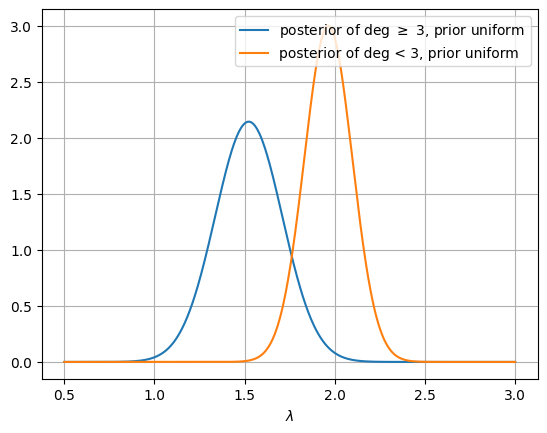
\includegraphics[width=0.6\linewidth]{figures/posterior_prior_uniform.png}
            \caption{So sánh phân phối hậu nghiệm tỷ lệ sinh của 2 nhóm phụ nữ khi phân phối tiên nghiệm của tỷ lệ sinh đều là phân phối đều}
            \label{fig:posterior_prior_uniform}
        \end{figure}
    
        Từ hình \ref{fig:posterior_prior_uniform}, ta nhận thấy tỷ lệ sinh trung bình của nhóm phụ nữ có trình độ văn hóa trên phổ thông có xu hướng nhỏ hơn tỷ lệ sinh trung bình của phụ nữ có trình độ văn hóa còn lại.
        Ta gọi kỳ vọng của phân phối hậu nghiệm của tỷ lệ sinh của nhóm có trình độ văn hóa trên phổ thông (DEG$\geq$3) là $\mu_1$ và kỳ vọng của phân phối hậu nghiệm của tỷ lệ sinh của nhóm có trình độ văn hóa còn lại là $\mu_2$.
        Ta xét bài toán kiểm định:
    
        \begin{equation*}
            \begin{cases}
                H_0: \mu_1 = \mu_2 \\
                H_1: \mu_1 < \mu_2
            \end{cases}
        \end{equation*}
    
        Do quan sát của hai nhóm phụ nữ đều lớn trên 30 (44 và 111), ta dùng tiêu chuẩn:
    
        \begin{equation*}
            T = \dfrac{\bar{\lambda}_1 - \bar{\lambda}_2}{\sqrt{s_1^2 + s_2^2}}
        \end{equation*}
    
        với $\bar{\lambda}_1=\dfrac{67}{44}, \bar{\lambda}_2=\dfrac{218}{111}$, $s_1^2=\dfrac{67}{44^2}, s_2^2=\dfrac{218}{111^2}$
        Ở công thức tiêu chuẩn kiểm định, ở các vị trí cho phương sai không có chia cho lực lượng của các nhóm vì ta đang tính trên phân phối hậu nghiệm, phương sai đã được tính từ các quan sát.
        Trong trường hợp thông thường, các giá trị phương sai $\dfrac{\sigma^2}{n}$ là phương sai của mẫu quan sát được.
    
        Ta có miền bác bỏ giả thiết $H_0$:
    
        \begin{equation*}
            B_{\beta}= \lbrace T: T < z_{\beta} \rbrace
        \end{equation*}
        với $\beta$ là mức ý nghĩa. Ta chọn mức ý nghĩa $\beta=0.05$, vậy $z_{0.05}\approx-1.6449$
    
        Ta tính $T=\dfrac{\dfrac{67}{44} - \dfrac{218}{111}}{\sqrt{\dfrac{67}{44^2} + \dfrac{218}{111^2}}}\approx-1.9294 \in B_{0.05}$
    
        Ta nhận thấy $T$ đã thuộc vào miền bác $H_0$, vậy nên ta bác bỏ $H_0$, chấp nhận $H_1$
    
        \item Trường hợp phân phối tiên nghiệm của tỷ lệ sinh là phân phối gamma $g(\lambda) = \text{gamma}(\lambda; r, \alpha)=\text{gamma}(\lambda; 2, 10)$ (ta chọn $r=2, \alpha=10$):
        
        Phân phối hậu nghiệm của tỷ lệ sinh của nhóm có trình độ văn hóa trên phổ thông (DEG$\geq$3) là:

        \begin{equation*}
            \begin{aligned}
                g(\lambda \vert X_1 =x_1, X_2=x_2, \dots, X_n=x_n) &= \text{gamma}\big(\lambda; 46, 76 \big) \\
                &\approx\mathcal{N}\Big(\dfrac{76}{46};\dfrac{76}{46^2})
            \end{aligned}
        \end{equation*}

        Phân phối hậu nghiệm của tỷ lệ sinh của nhóm có trình độ văn hóa còn lại (DEG$<$3) là:

        \begin{equation*}
            \begin{aligned}
                g(\lambda \vert X_1 =x_1, X_2=x_2, \dots, X_n=x_n) &= \text{gamma}\big(\lambda; 113, 227 \big) \\
                &\approx\mathcal{N}\Big(\dfrac{227}{113};\dfrac{227}{113^2})
            \end{aligned}
        \end{equation*}

        Ta vẽ phân phối hậu nghiệm của tỷ lệ sinh của hai nhóm phụ nữ khi phân phối tiên nghiệm
        là phân phối đều bằng đoạn code:

        \begin{python}
x = np.linspace(0.5, 3, 1000)

normal_approx_deg_geq_3 = normal_pdf_vector(x, (child_total_deg_geq_3 + alpha)/(n_deg_geq_3 + r), np.sqrt((child_total_deg_geq_3 + alpha)/((n_deg_geq_3 + r)**2)))
normal_approx_deg_less_3 = normal_pdf_vector(x, (child_total_deg_less_3 + alpha)/(n_deg_less_3 + r), np.sqrt((child_total_deg_less_3 + alpha)/((n_deg_less_3 + r)**2)))
            
plt.plot(x, normal_approx_deg_geq_3, label="posterior of deg $\geq$ 3, prior gamma", linestyle="solid")
plt.plot(x, normal_approx_deg_less_3, label="posterior of deg < 3, prior gamma", linestyle="solid")
plt.xlabel("$\lambda$")
plt.legend()
plt.grid()
plt.show()
        \end{python}

        \begin{figure}[h!]
            \centering
            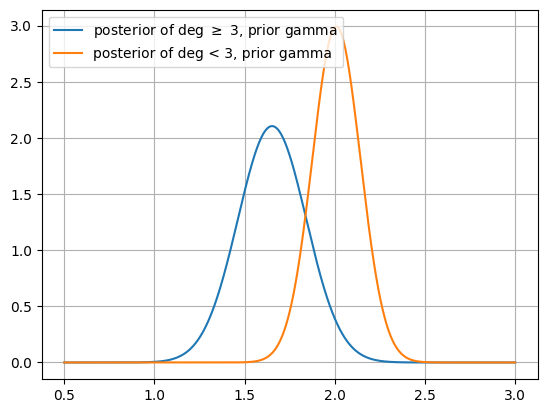
\includegraphics[width=0.6\linewidth]{figures/posterior_prior_gamma.png}
            \caption{So sánh phân phối hậu nghiệm tỷ lệ sinh của 2 nhóm phụ nữ khi phân phối tiên nghiệm của tỷ lệ sinh đều là phân phối gamma $g(\lambda)=\text{gamma}(\lambda; 2, 10)$}
            \label{fig:posterior_prior_gamma}
        \end{figure}
        

        Từ hình \ref{fig:posterior_prior_gamma}, ta nhận thấy tỷ lệ sinh trung bình của nhóm phụ nữ có trình độ văn hóa trên phổ thông có xu hướng nhỏ hơn tỷ lệ sinh trung bình của phụ nữ có trình độ văn hóa còn lại.
        Ta gọi kỳ vọng của phân phối hậu nghiệm của tỷ lệ sinh của nhóm có trình độ văn hóa trên phổ thông (DEG$\geq$3) là $\mu_1$ và kỳ vọng của phân phối hậu nghiệm của tỷ lệ sinh của nhóm có trình độ văn hóa còn lại là $\mu_2$.
        Ta xét bài toán kiểm định:
    
        \begin{equation*}
            \begin{cases}
                H_0: \mu_1 = \mu_2 \\
                H_1: \mu_1 < \mu_2
            \end{cases}
        \end{equation*}
    
        Do số quan sát của hai nhóm phụ nữ đều lớn trên 30 (44 và 111), ta dùng tiêu chuẩn:
    
        \begin{equation*}
            T = \dfrac{\bar{\lambda}_1 - \bar{\lambda}_2}{\sqrt{s_1^2 + s_2^2}}
        \end{equation*}
    
        với $\bar{\lambda}_1=\dfrac{76}{46}, \bar{\lambda}_2=\dfrac{227}{113}$, $s_1^2=\dfrac{76}{46^2}, s_2^2=\dfrac{227}{113^2}$
    
        Ta có miền bác bỏ giả thiết $H_0$:
    
        \begin{equation*}
            B_{\beta}= \lbrace T: T < z_{\beta} \rbrace
        \end{equation*}
        với $\beta$ là mức ý nghĩa. Ta chọn mức ý nghĩa $\beta=0.05$, vậy $z_{0.05}\approx-1.6449$
    
        Ta tính $T=\dfrac{\dfrac{76}{46} - \dfrac{227}{113}}{\sqrt{\dfrac{76}{46^2} + \dfrac{227}{113^2}}}\approx-1.5393 \notin B_{0.05}$

        Như vậy ta chưa có cơ sở bác bỏ $H_0$, ta chấp nhận giả thiết $H_0$, ta có thể xem tỷ lệ sinh của hai nhóm phụ nữ là như nhau.

        Ta nhận thấy khi phân phối tiên nghiệm của tỷ lệ sinh là phân phối gamma, thì sự khác biệt tỷ lệ sinh giữa hai nhóm phụ thuộc vào rất nhiều $r$ và $\alpha$.
        Trong trường hợp này $\alpha=10$ lớn hơn khá nhiều so với $r=2$ làm cho tỷ lệ sinh trung bình của nhóm 1 tăng nhiều hơn tương đối so với nhóm 2 vì vậy làm giảm giá trị của tiêu chuẩn kiểm định.
        Nếu như giá trị $r$ và $\alpha$ nhỏ hơn chỉ khoảng từ 1 đến 3 thì sự khác biệt về tỷ lệ sinh trung bình của hai nhóm không thay đổi nhiều so với trường hợp phân phối tiên nghiệm của tỷ lệ sinh là phân phối đều.

        \item Ta sẽ so sánh tỷ lệ sinh của 2 nhóm phụ nữ theo kiểm định từ dữ liệu hai nhóm phụ nữ
        
        Ta sẽ xét bài toán kiểm định từ việc tính tiêu chuẩn kiêm định trực tiếp từ mẫu:

        Do số quan sát mỗi nhóm phụ nữ đều lớn hơn 30 (44 và 111), mỗi biến $X_1, X_2, \dots, X_n$ độc lập và cùng tuân theo phân phối Poisson,
        theo luật số lớn $\bar{X} = \dfrac{X_1 + X_2 + \dots + X_n}{n}$ sẽ xấp xỉ phân phối chuẩn

        Ta xét bài toán kiểm định:

        \begin{equation*}
            \begin{cases}
                H_0: \mu_1 = \mu_2 \\
                H_1: \mu_1 < \mu_2
            \end{cases}
        \end{equation*}

        Do số quan sát của hai nhóm phụ nữ đều lớn trên 30 (44 và 111), ta dùng tiêu chuẩn:

        \begin{equation*}
            T = \dfrac{\bar{x} - \bar{y}}{\sqrt{\dfrac{s_1^2}{n_1} + \dfrac{s_2^2}{n_2}}}
        \end{equation*}

        với $\bar{x}$ là trung bình mẫu của nhóm 1, $\bar{y}$ là trung bình mẫu của nhóm 2,
        $s_1$ là phương sai mẫu của nhóm 1 và $s_2$ là phương sai mẫu của nhóm 2.

        Miền bác bỏ giả thiết $H_0$ là:

        \begin{equation*}
            B_{\beta}= \lbrace T: T < z_{\beta} \rbrace
        \end{equation*}
        với $\beta$ là mức ý nghĩa. Ta chọn mức ý nghĩa $\beta=0.05$, vậy $z_{0.05}\approx-1.6449$

        Ta tính $T$ bằng đoạn code sau:

        \begin{python}
observes_group_1 = df_deg_geq_3.CHILDS.to_numpy()
observes_group_2 = df_deg_less_3.CHILDS.to_numpy()

x_bar = np.mean(observes_group_1)
y_bar = np.mean(observes_group_2)

s_1 = np.sqrt(np.sum((observes_group_1 - x_bar)**2)/(observes_group_1.shape[0] - 1))
s_2 = np.sqrt(np.sum((observes_group_2 - y_bar)**2)/(observes_group_2.shape[0] - 1))

t = (x_bar - y_bar)/np.sqrt(s_1**2/n_deg_geq_3 + s_2**2/n_deg_less_3)
        \end{python}

        Ta tính được:

        \begin{equation*}
            T = \dfrac{\bar{x} - \bar{y}}{\sqrt{\dfrac{s_1^2}{n_1} + \dfrac{s_2^2}{n_2}}}=\dfrac{1.5 - 1.9550}{\sqrt{\dfrac{1.3721}{44} + \dfrac{1.8980}{111}}}\approx -2.0705 \in B_{0.05}
        \end{equation*}

        Ta nhận thấy $T$ đã thuộc vào miền bác $H_0$, vậy nên ta bác bỏ $H_0$, chấp nhận $H_1$.
    \end{itemize}

    \textbf{Nhận xét:} Ta nhận thấy giá trị của tiêu chuẩn kiểm định trong trường hợp xét phân phối hậu nghiệm tỷ lệ sinh khi phân phối tiên nghiệm tỷ lệ sinh là phân phối đều và trong trường hợp tính kiểm định thống kê từ mẫu, các kết quả kiểm định trong các trường hợp này khá gần nhau.
    Điều này cho ta thấy, tính kiểm định thống kê thông thường từ các mẫu xem khả năng xảy ra của các tỷ lệ sinh ban đầu là như nhau (phân phối đều).
    Nhưng trong trường hợp phân phối tiên nghiệm là phân phối gamma thì phân phối hậu nghiệm hay sự khác biệt giữa tỷ lệ sinh của hai nhóm phụ nữ phụ thuộc rất nhiều vào hai tham số $r$ và $\alpha$ của phân phối tiên nghiệm.
    
    \end{enumerate}
\end{loigiai}

\newpage
\begin{center}
    \section*{KẾT LUẬN}
\end{center}

Sau khi phân tích số liệu về tỷ lệ sinh của phụ nữ Mỹ ở độ tuổi 40 trong thập niên 1990 (YEAR $\geq$ 1990 \& AGE==40 \& FEMALE==1).
Có 02 nhóm phụ nữ được nghiên cứu là nhóm có trình độ văn hoá trên phổ thông (DEG $\geq$ 3) và nhóm còn lại, ta có một số kết luận sau:

\begin{itemize}
    \item Trong trường hợp phân phối tiên nghiệm của tỷ lệ sinh là đều hoặc phân phối gamma thì phân phối hậu nghiệm của tỷ lệ sinh cũng là gamma
    \item Khi số quan sát lớn và tổng số lượng trẻ em được sinh ra tương đối lớn thì phân phối hậu nghiệm của tỷ lệ sinh xấp xỉ chuẩn
    \item Trong trường hợp phân phối tiên nghiệm của tỷ lệ sinh là phân phối đều thì tỷ lệ sinh trung bình của nhóm phụ nữ có trình độ văn hóa trên phổ thông (DEG $\geq$ 3) nhỏ hơn tỷ lệ sinh trung bình của nhóm phụ nữ có trình độ văn hóa còn lại (DEG $<$ 3).
    \item Trong trường hợp phân phối tiên nghiệm của tỷ lệ sinh là phân phối $\text{gamma}(\lambda; r, \alpha)$ thì sự khác biệt giữa tỷ lệ sinh trung bình của hai nhóm phụ nữ phụ thuộc nhiều vào $r$ và $\alpha$.
    Trong trường hợp $r$ và $\alpha$ tương đối nhỏ (chỉ khoảng từ 1 đến 3) thì sự khác biệt về tỷ lệ sinh trung bình của hai nhóm không thay đổi nhiều so với trường hợp phân phối tiên nghiệm của tỷ lệ sinh là phân phối đều làm cho giá trị tiêu chuẩn kiểm định không khác nhiều giá trị tiêu chuẩn kiểm định trong trường hợp phân phối tiên nghiệm của tỷ lệ sinh là phân phối đều.
    
\end{itemize}

\newpage
\printbibliography[title={TÀI LIỆU THAM KHẢO}]


\end{document}